\documentclass[10pt, xcolor=table,aspectratio=169]{beamer}
\usepackage[square,sort,comma,numbers]{natbib}
\usefonttheme{professionalfonts}
% \usepackage{fourier}
\usepackage{epigraph}
% \beamerdefaultoverlayspecification{<+->}

% input defined packages
%%%%% NEW MATH DEFINITIONS %%%%%

\usepackage{amsmath,amsfonts,bm}
% for widebar
\makeatletter
\let\save@mathaccent\mathaccent
\newcommand*\if@single[3]{%
  \setbox0\hbox{${\mathaccent"0362{#1}}^H$}%
  \setbox2\hbox{${\mathaccent"0362{\kern0pt#1}}^H$}%
  \ifdim\ht0=\ht2 #3\else #2\fi
  }
%The bar will be moved to the right by a half of \macc@kerna, which is computed by amsmath:
\newcommand*\rel@kern[1]{\kern#1\dimexpr\macc@kerna}
%If there's a superscript following the bar, then no negative kern may follow the bar;
%an additional {} makes sure that the superscript is high enough in this case:
\newcommand*\widebar[1]{\@ifnextchar^{{\wide@bar{#1}{0}}}{\wide@bar{#1}{1}}}
%Use a separate algorithm for single symbols:
\newcommand*\wide@bar[2]{\if@single{#1}{\wide@bar@{#1}{#2}{1}}{\wide@bar@{#1}{#2}{2}}}
\newcommand*\wide@bar@[3]{%
  \begingroup
  \def\mathaccent##1##2{%
%Enable nesting of accents:
    \let\mathaccent\save@mathaccent
%If there's more than a single symbol, use the first character instead (see below):
    \if#32 \let\macc@nucleus\first@char \fi
%Determine the italic correction:
    \setbox\z@\hbox{$\macc@style{\macc@nucleus}_{}$}%
    \setbox\tw@\hbox{$\macc@style{\macc@nucleus}{}_{}$}%
    \dimen@\wd\tw@
    \advance\dimen@-\wd\z@
%Now \dimen@ is the italic correction of the symbol.
    \divide\dimen@ 3
    \@tempdima\wd\tw@
    \advance\@tempdima-\scriptspace
%Now \@tempdima is the width of the symbol.
    \divide\@tempdima 10
    \advance\dimen@-\@tempdima
%Now \dimen@ = (italic correction / 3) - (Breite / 10)
    \ifdim\dimen@>\z@ \dimen@0pt\fi
%The bar will be shortened in the case \dimen@<0 !
    \rel@kern{0.6}\kern-\dimen@
    \if#31
      \overline{\rel@kern{-0.6}\kern\dimen@\macc@nucleus\rel@kern{0.4}\kern\dimen@}%
      \advance\dimen@0.4\dimexpr\macc@kerna
%Place the combined final kern (-\dimen@) if it is >0 or if a superscript follows:
      \let\final@kern#2%
      \ifdim\dimen@<\z@ \let\final@kern1\fi
      \if\final@kern1 \kern-\dimen@\fi
    \else
      \overline{\rel@kern{-0.6}\kern\dimen@#1}%
    \fi
  }%
  \macc@depth\@ne
  \let\math@bgroup\@empty \let\math@egroup\macc@set@skewchar
  \mathsurround\z@ \frozen@everymath{\mathgroup\macc@group\relax}%
  \macc@set@skewchar\relax
  \let\mathaccentV\macc@nested@a
%The following initialises \macc@kerna and calls \mathaccent:
  \if#31
    \macc@nested@a\relax111{#1}%
  \else
%If the argument consists of more than one symbol, and if the first token is
%a letter, use that letter for the computations:
    \def\gobble@till@marker##1\endmarker{}%
    \futurelet\first@char\gobble@till@marker#1\endmarker
    \ifcat\noexpand\first@char A\else
      \def\first@char{}%
    \fi
    \macc@nested@a\relax111{\first@char}%
  \fi
  \endgroup
}
\makeatother

% Mark sections of captions for referring to divisions of figures
\newcommand{\figleft}{{\em (Left)}}
\newcommand{\figcenter}{{\em (Center)}}
\newcommand{\figright}{{\em (Right)}}
\newcommand{\figtop}{{\em (Top)}}
\newcommand{\figbottom}{{\em (Bottom)}}
\newcommand{\captiona}{{\em (a)}}
\newcommand{\captionb}{{\em (b)}}
\newcommand{\captionc}{{\em (c)}}
\newcommand{\captiond}{{\em (d)}}

% Highlight a newly defined term
\newcommand{\newterm}[1]{{\bf #1}}


% Figure reference, lower-case.
\def\figref#1{figure~\ref{#1}}
% Figure reference, capital. For start of sentence
\def\Figref#1{Figure~\ref{#1}}
\def\twofigref#1#2{figures \ref{#1} and \ref{#2}}
\def\quadfigref#1#2#3#4{figures \ref{#1}, \ref{#2}, \ref{#3} and \ref{#4}}
% Section reference, lower-case.
\def\secref#1{section~\ref{#1}}
% Section reference, capital.
\def\Secref#1{Section~\ref{#1}}
% Reference to two sections.
\def\twosecrefs#1#2{sections \ref{#1} and \ref{#2}}
% Reference to three sections.
\def\secrefs#1#2#3{sections \ref{#1}, \ref{#2} and \ref{#3}}
% Reference to an equation, lower-case.
\def\eqref#1{equation~\ref{#1}}
% Reference to an equation, upper case
\def\Eqref#1{Equation~\ref{#1}}
% A raw reference to an equation---avoid using if possible
\def\plaineqref#1{\ref{#1}}
% Reference to a chapter, lower-case.
\def\chapref#1{chapter~\ref{#1}}
% Reference to an equation, upper case.
\def\Chapref#1{Chapter~\ref{#1}}
% Reference to a range of chapters
\def\rangechapref#1#2{chapters\ref{#1}--\ref{#2}}
% Reference to an algorithm, lower-case.
\def\algref#1{algorithm~\ref{#1}}
% Reference to an algorithm, upper case.
\def\Algref#1{Algorithm~\ref{#1}}
\def\twoalgref#1#2{algorithms \ref{#1} and \ref{#2}}
\def\Twoalgref#1#2{Algorithms \ref{#1} and \ref{#2}}
% Reference to a part, lower case
\def\partref#1{part~\ref{#1}}
% Reference to a part, upper case
\def\Partref#1{Part~\ref{#1}}
\def\twopartref#1#2{parts \ref{#1} and \ref{#2}}

\def\ceil#1{\lceil #1 \rceil}
\def\floor#1{\lfloor #1 \rfloor}
\def\1{\bm{1}}
\newcommand{\train}{\mathcal{D}}
\newcommand{\valid}{\mathcal{D_{\mathrm{valid}}}}
\newcommand{\test}{\mathcal{D_{\mathrm{test}}}}

\def\eps{{\epsilon}}


% Random variables
\def\reta{{\textnormal{$\eta$}}}
\def\ra{{\textnormal{a}}}
\def\rb{{\textnormal{b}}}
\def\rc{{\textnormal{c}}}
\def\rd{{\textnormal{d}}}
\def\re{{\textnormal{e}}}
\def\rf{{\textnormal{f}}}
\def\rg{{\textnormal{g}}}
\def\rh{{\textnormal{h}}}
\def\ri{{\textnormal{i}}}
\def\rj{{\textnormal{j}}}
\def\rk{{\textnormal{k}}}
\def\rl{{\textnormal{l}}}
% rm is already a command, just don't name any random variables m
\def\rn{{\textnormal{n}}}
\def\ro{{\textnormal{o}}}
\def\rp{{\textnormal{p}}}
\def\rq{{\textnormal{q}}}
\def\rr{{\textnormal{r}}}
\def\rs{{\textnormal{s}}}
\def\rt{{\textnormal{t}}}
\def\ru{{\textnormal{u}}}
\def\rv{{\textnormal{v}}}
\def\rw{{\textnormal{w}}}
\def\rx{{\textnormal{x}}}
\def\ry{{\textnormal{y}}}
\def\rz{{\textnormal{z}}}

% Random vectors
\def\rvepsilon{{\mathbf{\epsilon}}}
\def\rvtheta{{\mathbf{\theta}}}
\def\rva{{\mathbf{a}}}
\def\rvb{{\mathbf{b}}}
\def\rvc{{\mathbf{c}}}
\def\rvd{{\mathbf{d}}}
\def\rve{{\mathbf{e}}}
\def\rvf{{\mathbf{f}}}
\def\rvg{{\mathbf{g}}}
\def\rvh{{\mathbf{h}}}
\def\rvu{{\mathbf{i}}}
\def\rvj{{\mathbf{j}}}
\def\rvk{{\mathbf{k}}}
\def\rvl{{\mathbf{l}}}
\def\rvm{{\mathbf{m}}}
\def\rvn{{\mathbf{n}}}
\def\rvo{{\mathbf{o}}}
\def\rvp{{\mathbf{p}}}
\def\rvq{{\mathbf{q}}}
\def\rvr{{\mathbf{r}}}
\def\rvs{{\mathbf{s}}}
\def\rvt{{\mathbf{t}}}
\def\rvu{{\mathbf{u}}}
\def\rvv{{\mathbf{v}}}
\def\rvw{{\mathbf{w}}}
\def\rvx{{\mathbf{x}}}
\def\rvy{{\mathbf{y}}}
\def\rvz{{\mathbf{z}}}

% Elements of random vectors
\def\erva{{\textnormal{a}}}
\def\ervb{{\textnormal{b}}}
\def\ervc{{\textnormal{c}}}
\def\ervd{{\textnormal{d}}}
\def\erve{{\textnormal{e}}}
\def\ervf{{\textnormal{f}}}
\def\ervg{{\textnormal{g}}}
\def\ervh{{\textnormal{h}}}
\def\ervi{{\textnormal{i}}}
\def\ervj{{\textnormal{j}}}
\def\ervk{{\textnormal{k}}}
\def\ervl{{\textnormal{l}}}
\def\ervm{{\textnormal{m}}}
\def\ervn{{\textnormal{n}}}
\def\ervo{{\textnormal{o}}}
\def\ervp{{\textnormal{p}}}
\def\ervq{{\textnormal{q}}}
\def\ervr{{\textnormal{r}}}
\def\ervs{{\textnormal{s}}}
\def\ervt{{\textnormal{t}}}
\def\ervu{{\textnormal{u}}}
\def\ervv{{\textnormal{v}}}
\def\ervw{{\textnormal{w}}}
\def\ervx{{\textnormal{x}}}
\def\ervy{{\textnormal{y}}}
\def\ervz{{\textnormal{z}}}

% Random matrices
\def\rmA{{\mathbf{A}}}
\def\rmB{{\mathbf{B}}}
\def\rmC{{\mathbf{C}}}
\def\rmD{{\mathbf{D}}}
\def\rmE{{\mathbf{E}}}
\def\rmF{{\mathbf{F}}}
\def\rmG{{\mathbf{G}}}
\def\rmH{{\mathbf{H}}}
\def\rmI{{\mathbf{I}}}
\def\rmJ{{\mathbf{J}}}
\def\rmK{{\mathbf{K}}}
\def\rmL{{\mathbf{L}}}
\def\rmM{{\mathbf{M}}}
\def\rmN{{\mathbf{N}}}
\def\rmO{{\mathbf{O}}}
\def\rmP{{\mathbf{P}}}
\def\rmQ{{\mathbf{Q}}}
\def\rmR{{\mathbf{R}}}
\def\rmS{{\mathbf{S}}}
\def\rmT{{\mathbf{T}}}
\def\rmU{{\mathbf{U}}}
\def\rmV{{\mathbf{V}}}
\def\rmW{{\mathbf{W}}}
\def\rmX{{\mathbf{X}}}
\def\rmY{{\mathbf{Y}}}
\def\rmZ{{\mathbf{Z}}}

% Elements of random matrices
\def\ermA{{\textnormal{A}}}
\def\ermB{{\textnormal{B}}}
\def\ermC{{\textnormal{C}}}
\def\ermD{{\textnormal{D}}}
\def\ermE{{\textnormal{E}}}
\def\ermF{{\textnormal{F}}}
\def\ermG{{\textnormal{G}}}
\def\ermH{{\textnormal{H}}}
\def\ermI{{\textnormal{I}}}
\def\ermJ{{\textnormal{J}}}
\def\ermK{{\textnormal{K}}}
\def\ermL{{\textnormal{L}}}
\def\ermM{{\textnormal{M}}}
\def\ermN{{\textnormal{N}}}
\def\ermO{{\textnormal{O}}}
\def\ermP{{\textnormal{P}}}
\def\ermQ{{\textnormal{Q}}}
\def\ermR{{\textnormal{R}}}
\def\ermS{{\textnormal{S}}}
\def\ermT{{\textnormal{T}}}
\def\ermU{{\textnormal{U}}}
\def\ermV{{\textnormal{V}}}
\def\ermW{{\textnormal{W}}}
\def\ermX{{\textnormal{X}}}
\def\ermY{{\textnormal{Y}}}
\def\ermZ{{\textnormal{Z}}}

% Vectors
\def\vzero{{\bm{0}}}
\def\vone{{\bm{1}}}
\def\vmu{{\bm{\mu}}}
\def\vtheta{{\bm{\theta}}}
\def\va{{\bm{a}}}
\def\vb{{\bm{b}}}
\def\vc{{\bm{c}}}
\def\vd{{\bm{d}}}
\def\ve{{\bm{e}}}
\def\vf{{\bm{f}}}
\def\vg{{\bm{g}}}
\def\vh{{\bm{h}}}
\def\vi{{\bm{i}}}
\def\vj{{\bm{j}}}
\def\vk{{\bm{k}}}
\def\vl{{\bm{l}}}
\def\vm{{\bm{m}}}
\def\vn{{\bm{n}}}
\def\vo{{\bm{o}}}
\def\vp{{\bm{p}}}
\def\vq{{\bm{q}}}
\def\vr{{\bm{r}}}
\def\vs{{\bm{s}}}
\def\vt{{\bm{t}}}
\def\vu{{\bm{u}}}
\def\vv{{\bm{v}}}
\def\vw{{\bm{w}}}
\def\vx{{\bm{x}}}
\def\vy{{\bm{y}}}
\def\vz{{\bm{z}}}

% Elements of vectors
\def\evalpha{{\alpha}}
\def\evbeta{{\beta}}
\def\evepsilon{{\epsilon}}
\def\evlambda{{\lambda}}
\def\evomega{{\omega}}
\def\evmu{{\mu}}
\def\evpsi{{\psi}}
\def\evsigma{{\sigma}}
\def\evtheta{{\theta}}
\def\eva{{a}}
\def\evb{{b}}
\def\evc{{c}}
\def\evd{{d}}
\def\eve{{e}}
\def\evf{{f}}
\def\evg{{g}}
\def\evh{{h}}
\def\evi{{i}}
\def\evj{{j}}
\def\evk{{k}}
\def\evl{{l}}
\def\evm{{m}}
\def\evn{{n}}
\def\evo{{o}}
\def\evp{{p}}
\def\evq{{q}}
\def\evr{{r}}
\def\evs{{s}}
\def\evt{{t}}
\def\evu{{u}}
\def\evv{{v}}
\def\evw{{w}}
\def\evx{{x}}
\def\evy{{y}}
\def\evz{{z}}

% Matrix
\def\mA{{\bm{A}}}
\def\mB{{\bm{B}}}
\def\mC{{\bm{C}}}
\def\mD{{\bm{D}}}
\def\mE{{\bm{E}}}
\def\mF{{\bm{F}}}
\def\mG{{\bm{G}}}
\def\mH{{\bm{H}}}
\def\mI{{\bm{I}}}
\def\mJ{{\bm{J}}}
\def\mK{{\bm{K}}}
\def\mL{{\bm{L}}}
\def\mM{{\bm{M}}}
\def\mN{{\bm{N}}}
\def\mO{{\bm{O}}}
\def\mP{{\bm{P}}}
\def\mQ{{\bm{Q}}}
\def\mR{{\bm{R}}}
\def\mS{{\bm{S}}}
\def\mT{{\bm{T}}}
\def\mU{{\bm{U}}}
\def\mV{{\bm{V}}}
\def\mW{{\bm{W}}}
\def\mX{{\bm{X}}}
\def\mY{{\bm{Y}}}
\def\mZ{{\bm{Z}}}
\def\mBeta{{\bm{\beta}}}
\def\mPhi{{\bm{\Phi}}}
\def\mLambda{{\bm{\Lambda}}}
\def\mSigma{{\bm{\Sigma}}}

% Tensor
\DeclareMathAlphabet{\mathsfit}{\encodingdefault}{\sfdefault}{m}{sl}
\SetMathAlphabet{\mathsfit}{bold}{\encodingdefault}{\sfdefault}{bx}{n}
\newcommand{\tens}[1]{\bm{\mathsfit{#1}}}
\def\tA{{\tens{A}}}
\def\tB{{\tens{B}}}
\def\tC{{\tens{C}}}
\def\tD{{\tens{D}}}
\def\tE{{\tens{E}}}
\def\tF{{\tens{F}}}
\def\tG{{\tens{G}}}
\def\tH{{\tens{H}}}
\def\tI{{\tens{I}}}
\def\tJ{{\tens{J}}}
\def\tK{{\tens{K}}}
\def\tL{{\tens{L}}}
\def\tM{{\tens{M}}}
\def\tN{{\tens{N}}}
\def\tO{{\tens{O}}}
\def\tP{{\tens{P}}}
\def\tQ{{\tens{Q}}}
\def\tR{{\tens{R}}}
\def\tS{{\tens{S}}}
\def\tT{{\tens{T}}}
\def\tU{{\tens{U}}}
\def\tV{{\tens{V}}}
\def\tW{{\tens{W}}}
\def\tX{{\tens{X}}}
\def\tY{{\tens{Y}}}
\def\tZ{{\tens{Z}}}


% Graph
\def\gA{{\mathcal{A}}}
\def\gB{{\mathcal{B}}}
\def\gC{{\mathcal{C}}}
\def\gD{{\mathcal{D}}}
\def\gE{{\mathcal{E}}}
\def\gF{{\mathcal{F}}}
\def\gG{{\mathcal{G}}}
\def\gH{{\mathcal{H}}}
\def\gI{{\mathcal{I}}}
\def\gJ{{\mathcal{J}}}
\def\gK{{\mathcal{K}}}
\def\gL{{\mathcal{L}}}
\def\gM{{\mathcal{M}}}
\def\gN{{\mathcal{N}}}
\def\gO{{\mathcal{O}}}
\def\gP{{\mathcal{P}}}
\def\gQ{{\mathcal{Q}}}
\def\gR{{\mathcal{R}}}
\def\gS{{\mathcal{S}}}
\def\gT{{\mathcal{T}}}
\def\gU{{\mathcal{U}}}
\def\gV{{\mathcal{V}}}
\def\gW{{\mathcal{W}}}
\def\gX{{\mathcal{X}}}
\def\gY{{\mathcal{Y}}}
\def\gZ{{\mathcal{Z}}}

% Sets
\def\sA{{\mathbb{A}}}
\def\sB{{\mathbb{B}}}
\def\sC{{\mathbb{C}}}
\def\sD{{\mathbb{D}}}
% Don't use a set called E, because this would be the same as our symbol
% for expectation.
\def\sF{{\mathbb{F}}}
\def\sG{{\mathbb{G}}}
\def\sH{{\mathbb{H}}}
\def\sI{{\mathbb{I}}}
\def\sJ{{\mathbb{J}}}
\def\sK{{\mathbb{K}}}
\def\sL{{\mathbb{L}}}
\def\sM{{\mathbb{M}}}
\def\sN{{\mathbb{N}}}
\def\sO{{\mathbb{O}}}
\def\sP{{\mathbb{P}}}
\def\sQ{{\mathbb{Q}}}
\def\sR{{\mathbb{R}}}
\def\sS{{\mathbb{S}}}
\def\sT{{\mathbb{T}}}
\def\sU{{\mathbb{U}}}
\def\sV{{\mathbb{V}}}
\def\sW{{\mathbb{W}}}
\def\sX{{\mathbb{X}}}
\def\sY{{\mathbb{Y}}}
\def\sZ{{\mathbb{Z}}}

% Entries of a matrix
\def\emLambda{{\Lambda}}
\def\emA{{A}}
\def\emB{{B}}
\def\emC{{C}}
\def\emD{{D}}
\def\emE{{E}}
\def\emF{{F}}
\def\emG{{G}}
\def\emH{{H}}
\def\emI{{I}}
\def\emJ{{J}}
\def\emK{{K}}
\def\emL{{L}}
\def\emM{{M}}
\def\emN{{N}}
\def\emO{{O}}
\def\emP{{P}}
\def\emQ{{Q}}
\def\emR{{R}}
\def\emS{{S}}
\def\emT{{T}}
\def\emU{{U}}
\def\emV{{V}}
\def\emW{{W}}
\def\emX{{X}}
\def\emY{{Y}}
\def\emZ{{Z}}
\def\emSigma{{\Sigma}}

% entries of a tensor
% Same font as tensor, without \bm wrapper
\newcommand{\etens}[1]{\mathsfit{#1}}
\def\etLambda{{\etens{\Lambda}}}
\def\etA{{\etens{A}}}
\def\etB{{\etens{B}}}
\def\etC{{\etens{C}}}
\def\etD{{\etens{D}}}
\def\etE{{\etens{E}}}
\def\etF{{\etens{F}}}
\def\etG{{\etens{G}}}
\def\etH{{\etens{H}}}
\def\etI{{\etens{I}}}
\def\etJ{{\etens{J}}}
\def\etK{{\etens{K}}}
\def\etL{{\etens{L}}}
\def\etM{{\etens{M}}}
\def\etN{{\etens{N}}}
\def\etO{{\etens{O}}}
\def\etP{{\etens{P}}}
\def\etQ{{\etens{Q}}}
\def\etR{{\etens{R}}}
\def\etS{{\etens{S}}}
\def\etT{{\etens{T}}}
\def\etU{{\etens{U}}}
\def\etV{{\etens{V}}}
\def\etW{{\etens{W}}}
\def\etX{{\etens{X}}}
\def\etY{{\etens{Y}}}
\def\etZ{{\etens{Z}}}

% The true underlying data generating distribution
\newcommand{\pdata}{p_{\rm{data}}}
% The empirical distribution defined by the training set
\newcommand{\ptrain}{\hat{p}_{\rm{data}}}
\newcommand{\Ptrain}{\hat{P}_{\rm{data}}}
% The model distribution
\newcommand{\pmodel}{p_{\rm{model}}}
\newcommand{\Pmodel}{P_{\rm{model}}}
\newcommand{\ptildemodel}{\tilde{p}_{\rm{model}}}
% Stochastic autoencoder distributions
\newcommand{\pencode}{p_{\rm{encoder}}}
\newcommand{\pdecode}{p_{\rm{decoder}}}
\newcommand{\precons}{p_{\rm{reconstruct}}}

\newcommand{\laplace}{\mathrm{Laplace}} % Laplace distribution

\newcommand{\E}{\mathbb{E}}
\newcommand{\Ls}{\mathcal{L}}
% \newcommand{\R}{\mathbb{R}}
\newcommand{\emp}{\tilde{p}}
\newcommand{\lr}{\alpha}
\newcommand{\reg}{\lambda}
\newcommand{\rect}{\mathrm{rectifier}}
\newcommand{\softmax}{\mathrm{softmax}}
\newcommand{\sigmoid}{\sigma}
\newcommand{\softplus}{\zeta}
\newcommand{\KL}{D_{\mathrm{KL}}}
\newcommand{\Var}{\mathrm{Var}}
\newcommand{\standarderror}{\mathrm{SE}}
\newcommand{\Cov}{\mathrm{Cov}}
% Wolfram Mathworld says $L^2$ is for function spaces and $\ell^2$ is for vectors
% But then they seem to use $L^2$ for vectors throughout the site, and so does
% wikipedia.
\newcommand{\normlzero}{L^0}
\newcommand{\normlone}{L^1}
\newcommand{\normltwo}{L^2}
\newcommand{\normlp}{L^p}
\newcommand{\normmax}{L^\infty}

\newcommand{\parents}{Pa} % See usage in notation.tex. Chosen to match Daphne's book.

\DeclareMathOperator*{\argmax}{arg\,max}
\DeclareMathOperator*{\argmin}{arg\,min}

% \DeclareMathOperator{\sign}{sign}
% \DeclareMathOperator{\Tr}{Tr}
\let\ab\allowbreak

\newcommand{\ones}{\mathbf 1}
\newcommand{\reals}{{\mathbb{R}}}
\newcommand{\integers}{{\mbox{\bf Z}}}
\newcommand{\symm}{{\mbox{\bf S}}}  % symmetric matrices

\newcommand{\nullspace}{{\mathcal N}}
\newcommand{\range}{{\mathcal R}}
\newcommand{\Rank}{\mathop{\bf Rank}}
\newcommand{\Tr}{\mathop{\bf Tr}}
\newcommand{\diag}{\mathop{\bf diag}}
\newcommand{\card}{\mathop{\bf card}}
\newcommand{\rank}{\mathop{\bf rank}}
\newcommand{\conv}{\mathop{\bf conv}}
\newcommand{\prox}{\mathbf{prox}}


\newcommand{\xmark}{\text{\ding{55}}}
\newcommand{\cmark}{\text{\ding{51}}}

\newcommand{\smallfont}[1]{{\small#1}}
\newcommand{\dquote}[1]{``#1"}
% color
\newcommand{\cred}[1]{{\color{red}#1}}
\newcommand{\cblue}[1]{{\color{blue}#1}}
\newcommand{\blue}[1]{\textcolor[rgb]{0.00,0.00,1.00}{#1}}
\newcommand{\green}[1]{\textcolor[rgb]{0.00,0.50,0.00}{#1}}

\newcommand{\Expect}{\mathop{\bf E{}}}
\newcommand{\Prob}{\mathop{\bf Prob}}
\newcommand{\Co}{{\mathop {\bf Co}}} % convex hull
\newcommand{\dist}{\mathop{\bf dist{}}}
\newcommand{\epi}{\mathop{\bf epi}} % epigraph
\newcommand{\Vol}{\mathop{\bf vol}}
\newcommand{\dom}{\mathop{\bf dom}} % domain
\newcommand{\intr}{\mathop{\bf int}}
\newcommand{\sign}{\mathop{\bf sign}}
\newcommand{\avg}{\operatorname{avg}}

\newcommand{\cf}{{\it cf.}}
\newcommand{\eg}{{\it e.g.}}
\newcommand{\ie}{{\it i.e.}}
\newcommand{\etc}{{\it etc.}}

\newcommand{\tra}{\mathrm{tr}}

% \usepackage[utf8]{inputenc} % allow utf-8 input
%\usepackage[T1]{fontenc}    % use 8-bit T1 fonts
%\usepackage{hyperref}       % hyperlinks
\usepackage{url}            % simple URL typesetting
\usepackage{booktabs}       % professional-quality tables
\usepackage{amsfonts}       % blackboard math symbols
\usepackage{nicefrac}       % compact symbols for 1/2, etc.
\usepackage{microtype}      % microtypogrhy
\usepackage{natbib}
\usepackage{enumerate}
%\usepackage{enumitem}
\usepackage{hhline}
\usepackage{makecell}
\usepackage{pifont}
\usepackage{tcolorbox}
\usepackage{color}
\usepackage{cancel}

% use Times
%\usepackage{times}
% For figures
\usepackage{graphicx} % more modern
%\usepackage{epsfig} % less modern
%\usepackage{subfigure}
\usepackage{caption}
\usepackage{subcaption}
% For citations
\usepackage{amsmath}
\usepackage{amsthm}
\usepackage{amssymb}
\usepackage{tikz}
\usepackage{xcolor}
\usetikzlibrary{arrows}

\allowdisplaybreaks

%for fonts
\usepackage{mathrsfs}

% For algorithms
\usepackage{algorithm}
\usepackage{algorithmic}
% \usepackage[noend]{algpseudocode}
\usepackage{hyperref}
\usepackage{bm}
%\usepackage{todonotes}


%For theorems
\allowdisplaybreaks

\renewcommand{\algorithmicrequire}{\textbf{Input:}}
\renewcommand{\algorithmicensure}{\textbf{Output:}}

%for convinience
\newcommand{\RR}{\mathbb{R}}
\newcommand{\vct}{\boldsymbol }
%\newcommand{\mat}{\mathbf}
\newcommand{\rnd}{\mathsf}
\newcommand{\ud}{\mathrm d}
\newcommand{\nml}{\mathcal{N}}
\newcommand{\loss}{\mathcal{L}}
\newcommand{\hinge}{\mathcal{R}}
\newcommand{\kl}{\mathrm{KL}}
\newcommand{\cov}{\mathrm{cov}}
\newcommand{\dir}{\mathrm{Dir}}
\newcommand{\mult}{\mathrm{Mult}}
\newcommand{\err}{\mathrm{err}}
\newcommand{\sgn}{\mathrm{sgn}}
%\renewcommand{\span}{\mathrm{span}}
% \newcommand{\argmin}{\mathrm{argmin}}
% \newcommand{\argmax}{\mathrm{argmax}}
\newcommand{\poly}{\mathrm{poly}}
% \newcommand{\rank}{\mathrm{rank}}
% \newcommand{\conv}{\mathrm{conv}}
%\newcommand{\E}{\mathbb{E}}
% \newcommand{\diag}{\mat{diag}}
\newcommand{\acc}{\mathrm{acc}}

\newcommand{\leftabs}{\left\vert}
\newcommand{\rightabs}{\right\vert}
\newcommand{\leftnorm}{\left\Vert}
\newcommand{\rightnorm}{\right\Vert}

\newcommand{\aff}{\mathrm{aff}}
% \newcommand{\range}{\mathrm{Range}}
\newcommand{\Sgn}{\mathrm{sign}}

\newcommand{\hit}{\mathrm{hit}}
\newcommand{\cross}{\mathrm{cross}}
\newcommand{\Left}{\mathrm{left}}
\newcommand{\Right}{\mathrm{right}}
\newcommand{\Mid}{\mathrm{mid}}
\newcommand{\bern}{\mathrm{Bernoulli}}
\newcommand{\ols}{\mathrm{ols}}
\newcommand{\tr}{\mathrm{tr}}
\newcommand{\opt}{\mathrm{opt}}
%\newcommand{\ridge}{\mathrm{ridge}}
\newcommand{\unif}{\mathrm{unif}}
\newcommand{\Image}{\mathrm{im}}
\newcommand{\Kernel}{\mathrm{ker}}
\newcommand{\supp}{\mathrm{supp}}
\newcommand{\pred}{\mathrm{pred}}
\newcommand{\distequal}{\stackrel{\mathbf{P}}{=}}
%\newcommand{\gege}{\textcircled{1}}
\newcommand{\gege}{{A(\vect{w},\vect{w}_*)}}
\newcommand{\gele}{{A(\vect{w},-\vect{w}_*)}}
\newcommand{\lele}{{A(-\vect{w},-\vect{w}_*)}}
\newcommand{\lege}{{A(-\vect{w},\vect{w}_*)}}
\newcommand{\firstlayer}{\mathbf{W}}
\newcommand{\firstlayerWN}{v}
\newcommand{\secondlayer}{a}
\newcommand{\inputvar}{\vect{x}}
\newcommand{\anglemat}{\mathbf{\Phi}}
\newcommand{\holder}{H\"{o}lder }
\newcommand{\real}{\mathbb{R}}
\newcommand{\approxerr}{\delta}

\def\R{\mathbb{R}}
\def\Z{\mathbb{Z}}
\def\cA{\mathcal{A}}
\def\cB{\mathcal{B}}
\def\cD{\mathcal{D}}
\def\cE{\mathcal{E}}
\def\cF{\mathcal{F}}
\def\cG{\mathcal{G}}
\def\cH{\mathcal{H}}
\def\cS{\mathcal{S}}
\def\cI{\mathcal{I}}
\def\cL{\mathcal{L}}
\def\cM{\mathcal{M}}
\def\cN{\mathcal{N}}
\def\cP{\mathcal{P}}
\def\cS{\mathcal{S}}
\def\cT{\mathcal{T}}
\def\cV{\mathcal{V}}
\def\cW{\mathcal{W}}
\def\cZ{\mathcal{Z}}
\def\SS{\mathbb{S}}
\def\NN{\mathbb{N}}
\def\bP{\mathbf{P}}
\def\TV{\mathrm{TV}}
\def\MSE{\mathrm{MSE}}

\def\vw{\mathbf{w}}
\def\va{\mathbf{a}}
\def\vZ{\mathbf{Z}}

\newcommand{\mat}[1]{#1}
\newcommand{\vect}[1]{#1}
\newcommand{\norm}[1]{\left\|#1\right\|}
\newcommand{\normop}[1]{\left\|#1\right\|_{\mathrm{op}}}
\newcommand{\simplex}{\triangle}
\newcommand{\abs}[1]{\left|#1\right|}
\newcommand{\expect}{\mathbb{E}}
\newcommand{\prob}{\mathbb{P}}
% \newcommand{\prox}[2]{\textbf{Prox}_{#1}\left\{#2\right\}}
\newcommand{\event}[1]{\mathscr{#1}}
\newcommand{\set}[1]{#1}
\newcommand{\diff}{\text{d}}
\newcommand{\difference}{\triangle}
\newcommand{\inputdist}{\mathcal{Z}}
\newcommand{\indict}{\mathbb{I}}
\newcommand{\rotmat}{\mathbf{R}}
\newcommand{\normalize}[1]{\overline{#1}}
\newcommand{\vectorize}[1]{\text{vec}\left(#1\right)}
\newcommand{\vclass}{\mathcal{G}}
\newcommand{\pclass}{\Pi}
\newcommand{\qclass}{\mathcal{Q}}
\newcommand{\rclass}{\mathcal{R}}
\newcommand{\classComplexity}[2]{N_{class}(#1,#2)}
\newcommand{\cclass}{\mathcal{F}}
\newcommand{\gclass}{\mathcal{G}}
\newcommand{\pthres}{p_{thres}}
\newcommand{\ethres}{\epsilon_{thres}}
\newcommand{\eclass}{\epsilon_{class}}
\newcommand{\states}{\mathcal{S}}
\newcommand{\trans}{P}
\newcommand{\lowprobstate}{\psi}
\newcommand{\actions}{\mathcal{A}}
\newcommand{\contexts}{\mathcal{X}}
\newcommand{\edges}{\mathcal{E}}
\newcommand{\variance}{\text{Var}}
\newcommand{\params}{\vect{w}}

\newcommand{\relu}[1]{\sigma\left(#1\right)}
\newcommand{\reluder}[1]{\sigma'\left(#1\right)}
\newcommand{\act}[1]{\sigma\left(#1\right)}

\newtheorem{thm}{Theorem}
% \newtheorem{thm}{Theorem}
\newtheorem{lem}{Lemma}
% Thm -> corollary 
\newtheorem{cor}{Corollary}
\newtheorem{prop}{Proposition}
\newtheorem{asmp}{Assumption}
\newtheorem{defn}{Definition}
\newtheorem{oracle}{Oracle}
% \newtheorem{fact}{Fact}[section]
\newtheorem{conj}{Conjecture}
\newtheorem{rem}{Remark}
% \newtheorem{example}{Example}[section]
\newtheorem{condition}{Condition}



\usepackage{bbm}

% For line space
\usepackage{float}
\usepackage{setspace}
\linespread{1.2}
\usepackage{tabularx,ragged2e,booktabs}
\usepackage{diagbox}
\usepackage{ulem}

% \usepackage[font=small,labelfont=bf]{caption}
% \usepackage{subcaption}

\usepackage{caption}
\captionsetup[figure]{labelformat=empty}

\usepackage{setspace}
%\onehalfspacing
\setlength\abovedisplayskip{0pt}
\newcommand{\bigangle}[1]{{\langle#1\rangle}}

\usepackage[USenglish]{babel}
\usepackage[nodayofweek,level]{datetime}

\newcommand{\mydate}{\formatdate{18}{06}{2020}}

%\usepackage{cleveref}

%% formatting
\setbeamercovered{transparent}
% \setbeamertemplate{theorems}[numbered]
\setbeamertemplate{theorems}[ams style] 

\mode<presentation>
{
\usetheme{default}
}
\setbeamertemplate{navigation symbols}{}
\usecolortheme[rgb={0.13,0.28,0.59}]{structure}
\setbeamertemplate{itemize subitem}{--}
\setbeamertemplate{frametitle} {
	\begin{center}
	  {\large\bf \insertframetitle}
	\end{center}
}
\setbeamerfont{block title}{size=\normalsize}

\newcommand\footlineon{
  \setbeamertemplate{footline} {
    \begin{beamercolorbox}[ht=2.5ex,dp=1.125ex,leftskip=.8cm,rightskip=.6cm]{structure}
      \footnotesize \insertsection
      \hfill
      {\insertframenumber\,/\,\inserttotalframenumber}
    \end{beamercolorbox}
    \vskip 0.45cm
  }
}
\footlineon

\AtBeginSection[] 
{ 
	\begin{frame}<beamer> 
		\frametitle{Outline} 
		\tableofcontents[currentsection,currentsubsection] 
	\end{frame} 
}

\AtBeginSubsection[] 
{ 
	\begin{frame}<beamer> 
		\frametitle{Outline} 
		\tableofcontents[currentsection,currentsubsection] 
	\end{frame} 
} 


%% begin presentation

\title{\large \bfseries Bias and Fairness in Machine Learning}
% \subtitle{Statistics, Optimization and Reinforcement Learning}
\author{Shaokui Wei \\\href{mailto:shaokuiwei@link.cuhk.edu.cn}{shaokuiwei@link.cuhk.edu.cn}
}
\institute{School of Data Science\\The Chinese University of Hong Kong, Shenzhen, China}

%\date{}

\makeatletter
\let\@@magyar@captionfix\relax 
\makeatother

\begin{document}

\frame{
	\thispagestyle{empty}
	\titlepage
}
%%%%%%%%%%%%%%%%%%%%%%%%%%%%%%%%%%%%%%%%%%%%%%%%%%%%%%%%%%%%%%%
\section{Motivation}
\begin{frame}{Motivation}
	Examples of unfairness in Machine Learning:
	\begin{itemize}
		\item Unfairness in deep Abnormal Detection \cite{zhang2021towards}:
		      \begin{figure}[t]
			      \begin{center}
				      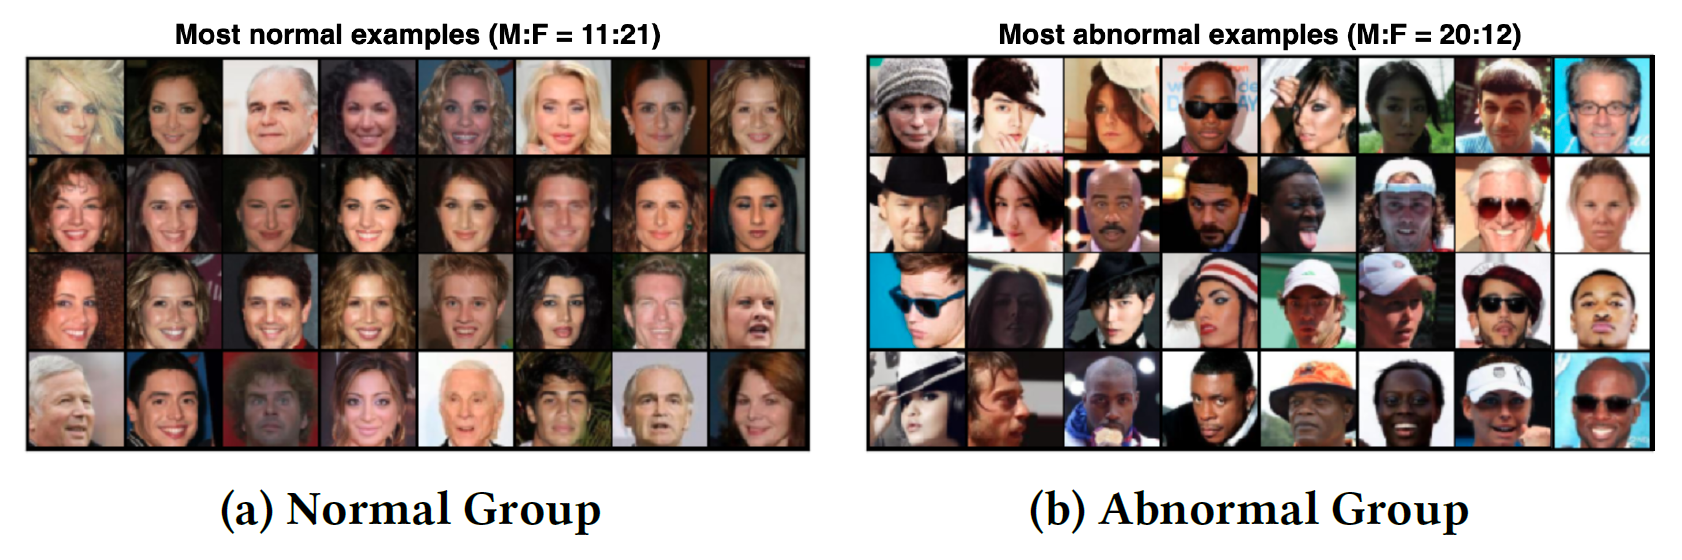
\includegraphics[width=0.8\columnwidth]{./figs/abnormal.png}
			      \end{center}
			      \caption{The top 32 normal instances and top 32 abnormal instances
				      discovered by deep SVDD on celebA data set are visualized. We see that the normal group is dominated by females while the abnormal
				      group is dominated by males.}
		      \end{figure}
	\end{itemize}

\end{frame}

\begin{frame}{Motivation}
	Examples of unfairness in Machine Learning:
	\begin{itemize}
		\item Unfairness in Correctional Offender Management Profiling for Alternative Sanctions (COMPAS) \cite{mehrabi2021survey}:

		      COMPAS is more likely to have higher false positive rates for African-American offenders than Caucasian offenders in falsely predicting them to be at a higher risk of recommitting a crime or recidivism.
	\end{itemize}

\end{frame}

\begin{frame}{Motivation}
	Examples of unfairness in Machine Learning:
	\begin{itemize}
		\item  \textbf{Illustrative example:} Consider the task to recognize the presence of wearing a hat. Suppose in the real world wearing a hat is correlated with wearing glasses. This correlation may be reflected in the training data, and a classifier trained to recognize a hat may rely on the presence of glasses. Consequently, the classifier may fail to recognize a hat in the absence of glasses, and vice versa \cite{ramaswamy2021fair}.
	\end{itemize}

\end{frame}
%%%%%%%%%%%%%%%%%%%%%%%%%%%%%%%%%%%%%%%%%%%%%%%%%%%%%%%%%%%%%%%
\section{Criteria of Fairness}

\begin{frame}{Terminologys}
	\begin{itemize}
		\item \textbf{Favorable label}:  A label whose value corresponds to an outcome that provides an advantage to the recipient.
		\item \textbf{Protected attribute}: An attribute that partitions a population into groups that have parity in terms of benefit received.
		\item \textbf{Privileged value}: A privileged value of a protected attribute indicates a group that has historically been at a systematic advantage.
		\item \textbf{Group Fairness}: Groups defined by protected attributes receive similar treatments or outcomes.
		\item \textbf{Individual fairness}: Similar individuals receive similar treatments or outcomes.
		\item \textbf{Fairness metric/criteria}: A quantification of unwanted bias in training data or models.
	\end{itemize}

\end{frame}

\begin{frame}{Criteria of Fairness}
	An algorithm is fair if it satisfies one specific criteria of fairness.
	Many fairness criterias have been proposed over the years and most of the proposed fairness criterias are properties of the joint
	distribution of the sensitive (projected) attribute $A$, remaining attributes $X$, the target label $Y$, and the	predicated label $\hat{Y}$. Here we assume that $Y, A\in \{0,1\}$ and give the definition of some popular criterias \cite{dunkelau2019fairness}. More criterias can be found in Section~\ref{app}.
	\begin{definition}[Independence]
		All groups experience the same acceptance rate.
		$$ P(\hat{Y}=1|A=0)=P(\hat{Y}=1|A=1)$$
	\end{definition}
	Note: The intuition is that label is independent of certain attributes. But this criteria ignores the distribution of label in each group.

\end{frame}

\begin{frame}{Criteria of Fairness}
	\begin{definition}[Separation]
		All groups experience the same true positive rate and the same false positive rate
		$$ P(\hat{Y}=1|A=0,Y=1)=P(\hat{Y}=1|A=1,Y=1)$$
		$$ P(\hat{Y}=1|A=0,Y=0)=P(\hat{Y}=1|A=1,Y=0)$$
	\end{definition}
	\begin{definition}[Sufficiency]
		All groups experience the same parity of positive/negative predictive values.
		$$ P(Y=1|A=0,\hat{Y}=1)=P(Y=1|A=1,\hat{Y}=1)$$
		$$ P(Y=1|A=0,\hat{Y}=0)=P(Y=1|A=1,\hat{Y}=0)$$
	\end{definition}

\end{frame}

\begin{frame}{Criteria of Fairness}
	In some applications it is desirable to be able to interpret the values of the score functions as probabilities.
	\begin{definition}[Calibration]
		Given a score function $R$, the calibration is
		$$ P(Y=1|A=0,R=r)=P(Y=1|A=1,R=r)=r, \quad \forall r\in [0,1]$$
	\end{definition}

\end{frame}

\begin{frame}{Criteria of Fairness}
	\begin{figure}[t]
		\begin{center}
			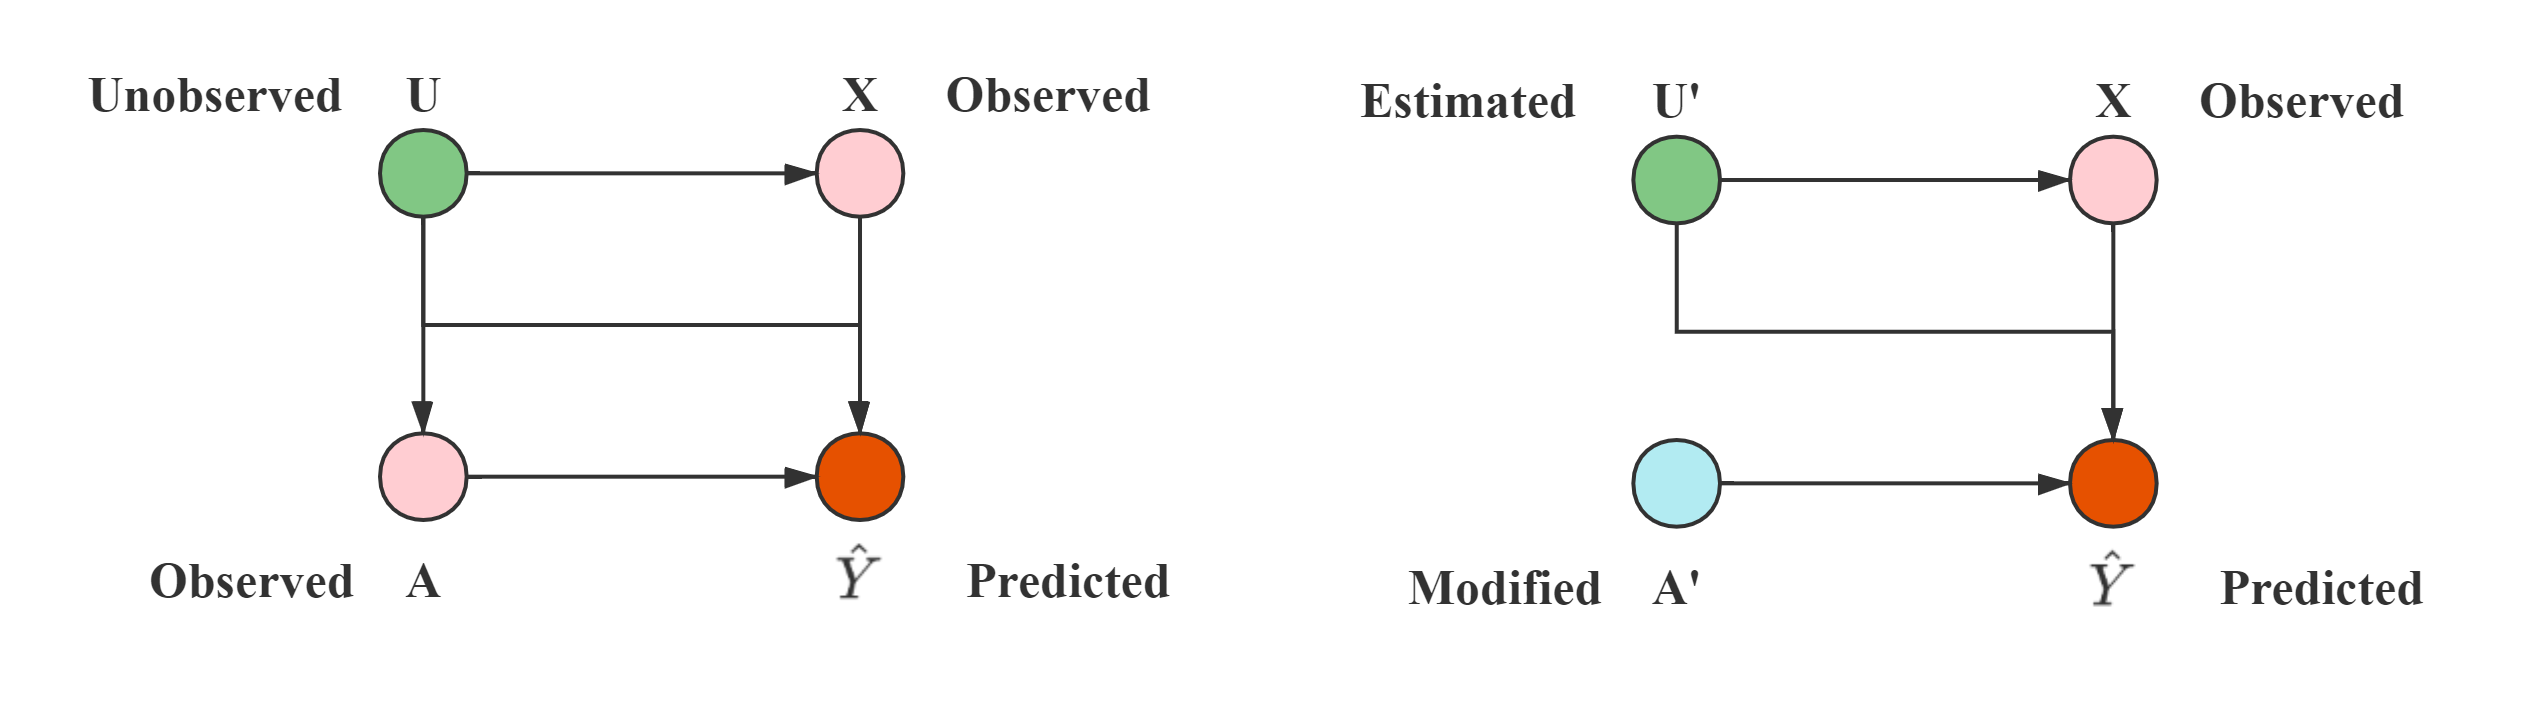
\includegraphics[width=0.8\columnwidth]{./figs/countf.png}
		\end{center}
		\caption{$\hat{Y}_{A\leftarrow a}(U)|X=x, A=a$ (Left) and $\hat{Y}_{A\leftarrow a'}(U)|X=x, A=a$ (Right)}
	\end{figure}
	\begin{definition}[Counterfactual Fairness \cite{russell2017worlds}]
		$$ P(\hat{Y}_{A\leftarrow a}(U)|X=x, A=a)=P(\hat{Y}_{A\leftarrow a'}(U)|X=x, A=a)$$
	\end{definition}

\end{frame}

%%%%%%%%%%%%%%%%%%%%%%%%%%%%%%%%%%%%%%%%%%%%%%%%%%%%%%%%%%%%%%%
\section{Source of Unfairness}

\begin{frame}{Data to Algorithm}
\begin{itemize}
	\item In this section, we will reiterate the most important sources of bias	and discrimination summarized in \cite{mehrabi2021survey}.
	
\end{itemize}

\end{frame}


\subsection{Bias}
\begin{frame}{Data to Algorithm}
	\begin{itemize}
		\item Measurement Bias: Measurement, or reporting bias arises from how we choose, utilize, and measure particular features.
		\item Omitted Variable Bias: Omitted variable bias occurs when one or more important variables	are left out of the model.
		\item Representation Bias: Representation bias arises from how we sample from a population during data collection process, e.g., lack of diversity.
		\item Aggregation Bias: Aggregation bias (or ecological fallacy) arises when false conclusions are drawn about individuals from observing the entire population.

	\end{itemize}

\end{frame}

\begin{frame}{Data to Algorithm}
	\begin{itemize}
		\item Sampling Bias: Sampling bias is similar to representation bias, and it arises due to non-random sampling of subgroups.
		\item Longitudinal Data Fallacy: Researchers analyzing temporal data must use longitudinal analysis to track cohorts over time to learn their behavior.
		\item Linking Bias: Linking bias arises when network attributes obtained from user connections, activities, or interactions differ and misrepresent the true behavior of the users.

	\end{itemize}

\end{frame}

\begin{frame}{Algorithm to User}
	\begin{itemize}
		\item Algorithmic Bias: Algorithmic bias is when the bias is not present in the input data and is added purely by the algorithm.
		\item User Interaction Bias: User Interaction bias is a type of bias that can not only be observant on the Web but also get triggered from two sources—the user interface and through the user itself by imposing his/her self-selected biased behavior and interaction.

	\end{itemize}

\end{frame}

\begin{frame}{Algorithm to User}
	\begin{itemize}
		\item Popularity Bias: Items that are more popular tend to be exposed more. However, popularity metrics are subject to manipulation—for example, by fake reviews or social bots.
		\item Emergent Bias: Emergent bias occurs as a result of use and interaction with real users. This bias arises as a result of change in population, cultural values, or societal knowledge usually some time after the completion of design.
		\item Evaluation Bias: Evaluation bias happens during model evaluation.

	\end{itemize}

\end{frame}

\begin{frame}{User to Data}
	\begin{itemize}
		\item Historical Bias: Historical bias is the already existing bias and socio-technical issues in the world and can seep into from the data generation process even given a perfect sampling and feature selection.
		\item Population Bias: Population bias arises when  statistics, demographics, representatives, and user characteristics are different in the user population of the platform from the original target population.
		\item Self-selection Bias: Self-selection bias is a subtype of the selection or sampling bias in which subjects of the research select themselves.


	\end{itemize}

\end{frame}

\begin{frame}{User to Data}
	\begin{itemize}
		\item Social Bias: Social bias happens when others’ actions affect our judgment.
		\item Behavioral Bias: Behavioral bias arises from different user behavior across platforms, contexts, or different dataset.
		\item Temporal Bias: Temporal bias arises from differences in populations and behaviors over time.
		\item Content Production Bias: Content Production bias arises from structural, lexical, semantic, and syntactic differences in the contents generated by users.

	\end{itemize}

\end{frame}

\subsection{Discrimination}

\begin{frame}{Type of Discrimination}
	Discrimination can be considered as	a source for unfairness that is due to human prejudice and stereotyping based on the sensitive
	attributes, which may happen intentionally or unintentionally.
	\begin{itemize}
		\item Explainable Discrimination: Differences in treatment and outcomes among different groups can be justified and explained via some attributes in some cases. In situations where these differences are justified and explained, it is not considered to be illegal discrimination and hence called explainable.
		\item Unexplainable Discrimination: In contrast to explainable discrimination, there is unexplainable discrimination in which the discrimination toward a group is unjustified and therefore considered illegal.
	\end{itemize}

\end{frame}


\begin{frame}{Type of Unexplainable Discrimination}
	\begin{itemize}
		\item Direct Discrimination: Direct discrimination happens when protected attributes of individuals explicitly result in non-favorable outcomes toward them.
		\item Indirect Discrimination: In indirect discrimination, individuals appear to be treated based on seemingly neutral and non-protected attributes; however, protected groups, or individuals, still get to be treated unjustly as a result of implicit effects from their protected attributes.
	\end{itemize}

\end{frame}

%%%%%%%%%%%%%%%%%%%%%%%%%%%%%%%%%%%%%%%%%%%%%%%%%%%%%%%%%%%%%%%
\section{Current Methods}
\begin{frame}{Overview of Methods}
	Generally, methods that target fairness in Machine Learning fall under three categories \cite{mehrabi2021survey}:
	\begin{itemize}
		\item Pre-processing: Pre-processing techniques try to transform the data so the underlying discrimination/bias is removed.
		\item In-processing: In-processing techniques try to modify and change state-of-the-art learning algorithms to remove discrimination during the model training process.
		\item Post-processing: Post-processing is performed after training by accessing a holdout set that was not involved during the training of the model.
	\end{itemize}
	We consider group fair binary classification problem to demonstrate different approaches. Assume that data $X$ has the protected attribute $Z \in \{0,1\}$ and label $Y \in \{0,1\}$.

\end{frame}

\subsection{Pre-processing}
\begin{frame}{Pre-processing}
	\begin{figure}[t]
		\begin{center}
			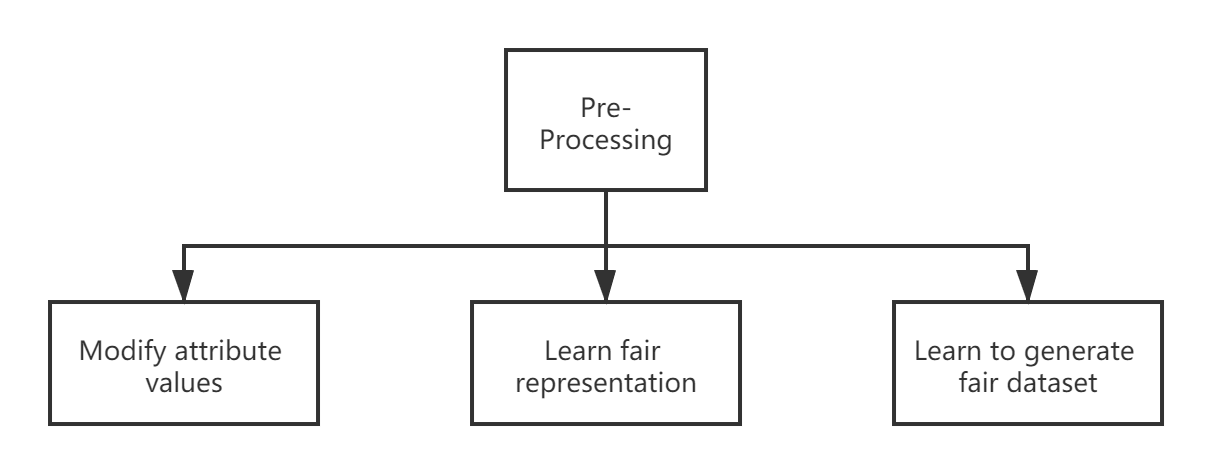
\includegraphics[width=0.8\columnwidth]{./figs/pp1m.png}
		\end{center}
		\caption{Overview of Pre-processing methods.}
	\end{figure}

\end{frame}
\begin{frame}{Unbiasing Data}
	\textbf{Relabelling (Massaging):} Take a number of individuals in the training data and change their ground truth values to ensure group fairness in dataset \cite{kamiran2009classifying}.
	\begin{itemize}
		\item Step 1: Compute the number $M$ of required modifications as\[			M=\eps\times \frac{|D_1|\times |D_0|}{|D_1|+|D_0|}
		      \]
		      where\[	\epsilon=P_1(Y=1)-P_0(Y=1) \quad D_1=\{X|Z=1\} \quad D_0=\{X|Z=0\}
		      \]
		\item Step 2: Sort the elements in $\{X\in D_0|Y=0\}$ in descending order and $\{X\in D_1|Y=1\}$ in ascending order by their probability to receive favorable label which is called 'rank'.
		\item Step 3: Labels of the top-M individuals in both sets get flipped.

	\end{itemize}

\end{frame}

\begin{frame}{Unbiasing Data}

	\begin{figure}[t]
		\begin{center}
			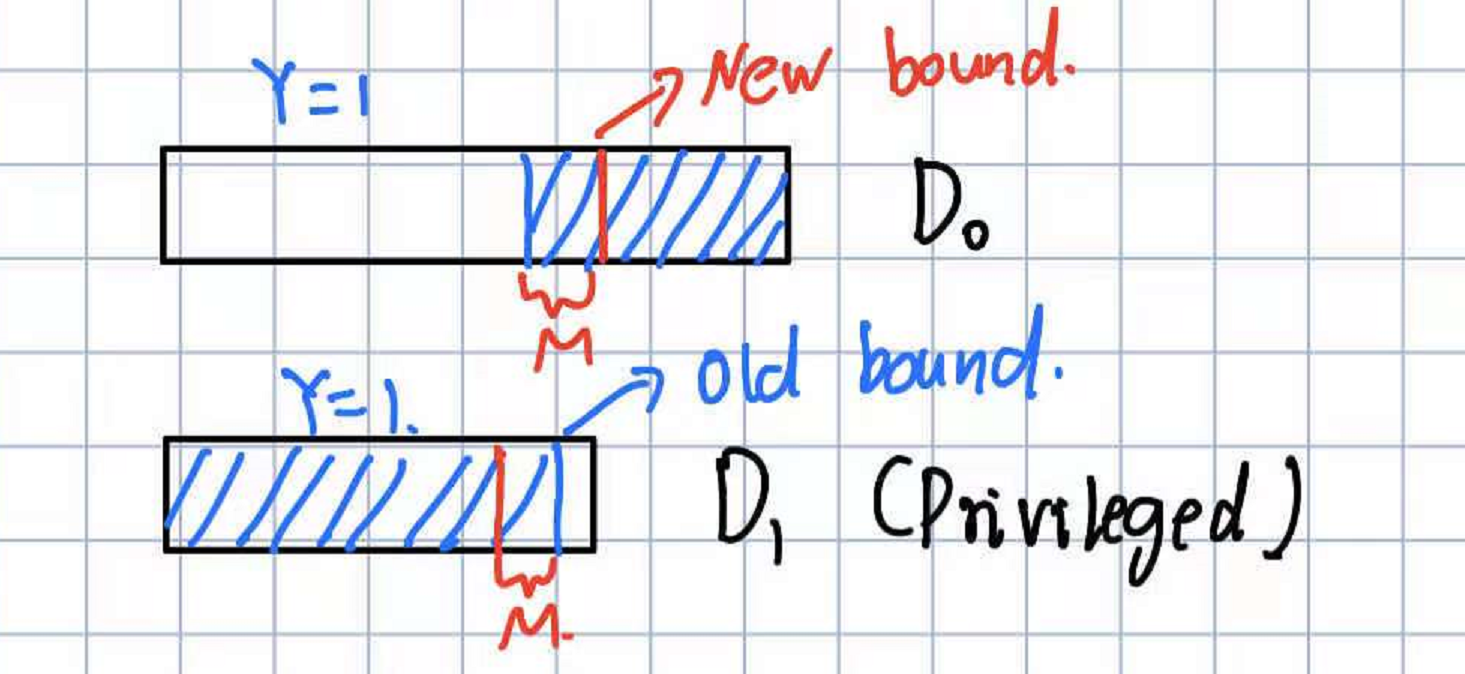
\includegraphics[width=0.3\columnwidth]{./figs/relabel.png}
		\end{center}
		\caption{}
		\begin{itemize}
			\item 	Question: What's the value of $M$?\\
			\item 	Answer: Solve the equation:
			      \[\frac{|D_0|\times P_0(Y=1)+M}{|D_0|}=\frac{|D_1|\times P_1(Y=1)-M}{|D_1|}
			      \]
			      Then,
			      \[M=\left(P_1(Y=1)-P_0(Y=1) \right)\times \frac{|D_1|\times |D_0|}{|D_1|+|D_0|}\]
		\end{itemize}
	\end{figure}

\end{frame}

\begin{frame}{Unbiasing Data}
	\textbf{Reweighing:} Assign a weight for each data to ensure group fairness in dataset \cite{kamiran2012data}.
	\begin{itemize}
		\item Each individual $X$ with $Y=y, Z=z$ is assigned a weight
		      \[W(y,z)=\frac{|\{X|Z=z\}|\times |\{X|Y=y\}|}{|D|\times |\{X|Z=z\cap Y=y\}|}\]
	\end{itemize}
	Note: Group fairness is achieved since
	\[\frac{|\{X|Z=z\cap Y=y\}|W(y,z)}{|\{X|Z=z\}|}=\frac{\{|X|Y=y|\}}{|D|}\]

\end{frame}

\begin{frame}{Unbiasing Data}
	\textbf{Preferential Sampling:} Duplicate or delete some data to ensure group fairness in dataset \cite{kamiran2012data}.
	\begin{itemize}
		\item Step 1: Let $D_z=\{(X,Y,Z)|Z=z\}$, $D^y=\{(X,Y,Z)|Y=y\}$ and $D_z^y=D_z\cap D^y$. Divide the dataset into four subsets $D_0^0, D_0^1, D_1^0$ and $D_1^1$.The expected cardinality of each subset is
		      \[C_z^y=\frac{|D_z|\times |D^y|}{|D|}\]
		\item Step 2: Sort subsets according to their ranks: $D_0^1, D_1^1$ ascending, $D_0^0, D_1^0$ descending.
		\item Step 3: Adjust each subset to match their respective $C_z^y$ values by either deleting the top elements or iteratively duplicating them.

	\end{itemize}

\end{frame}


\begin{frame}{Fair Representations}
	\textbf{Variational Fair Autoencoder:} Find a latent representation $\tilde{X}$
	of X which is minimally informative about Z yet maximally informative
	about Y \cite{louizos2015variational}.
	\begin{itemize}
		\item VAE: $\quad \quad \tilde{x} \sim p(\tilde{x}) \quad x\sim p_\theta(x|\tilde{x})$
		\item Fair VAE: $\tilde{x}\sim p(\tilde{x}) \quad x\sim p_\theta(x|\tilde{x},z)$
		\item Encourage separation between $\tilde{X}$ and Z by  encoding $Z$ into the decoder explicitly.
		\item Avoid keeping dependencies in the variational posterior $q(\tilde{X}|X,Z)$ by employing a maximum mean discrepancy term, i.e.,
		      \[l_{\text{MMD}}=\norm{E_{p(x|z=0)}[E_{q(\tilde{x}|x,z=0)}(\phi(\tilde{x}))]-E_{p(x|z=1)}[E_{q(\tilde{x}|x,z=1)}(\phi(\tilde{x}))]}^2\]
		      where $\phi $ is an empirical statistic.
	\end{itemize}


\end{frame}

\begin{frame}{Learn to Generate Fair Data}
	\begin{figure}[t]
		\begin{center}
			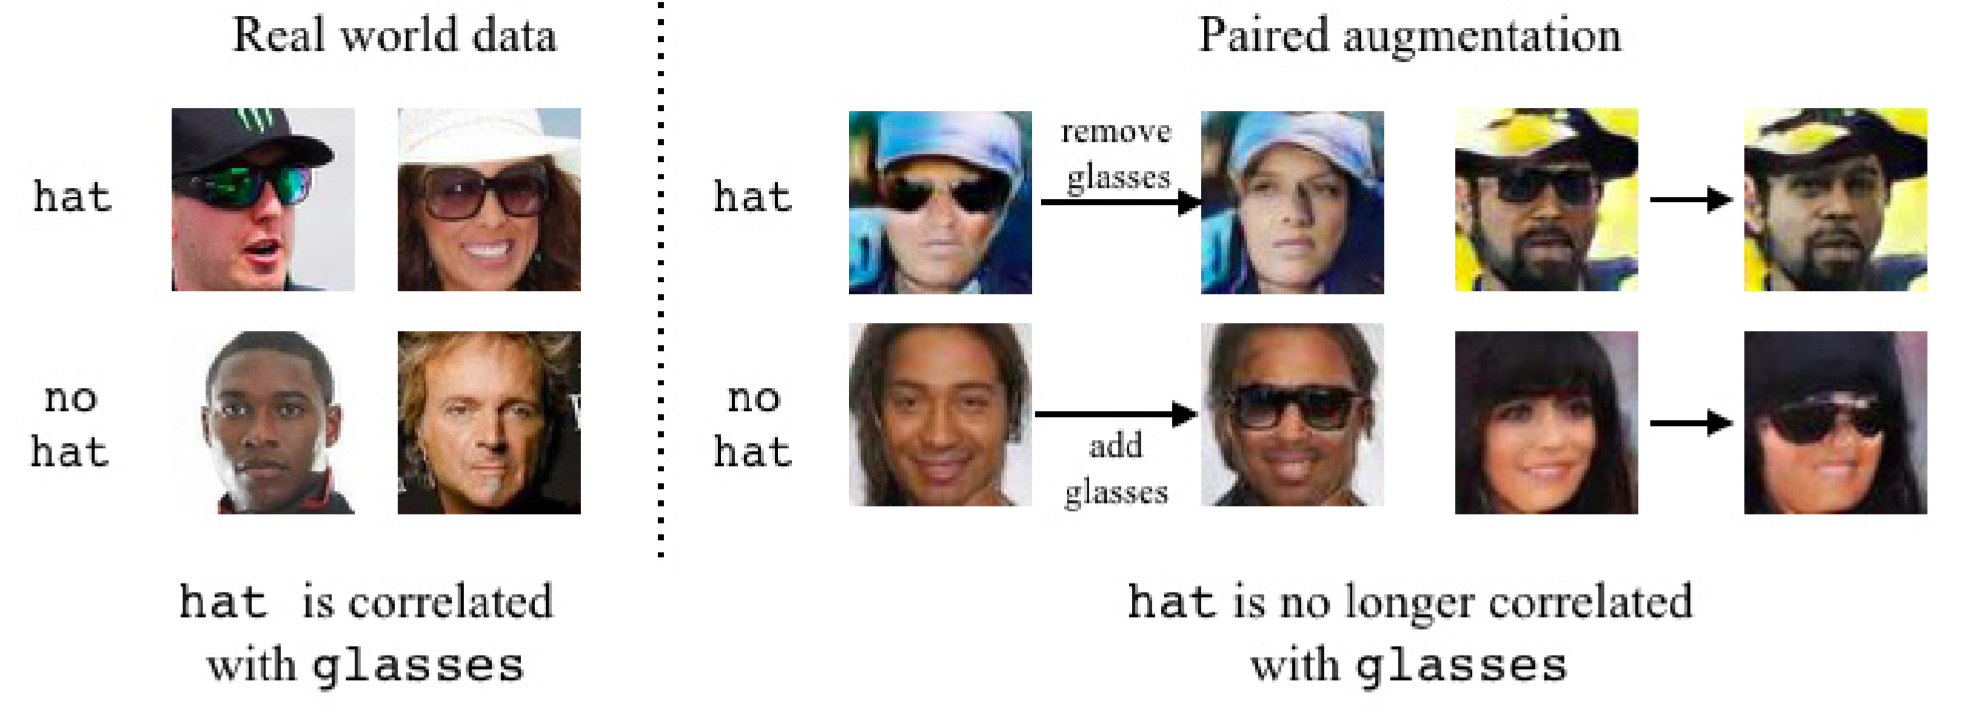
\includegraphics[width=0.8\columnwidth]{./figs/hat_gan.png}
		\end{center}
		\caption{Augment dataset using Generative Adversarial Networks (GANs) to removes the correlation between glass and hat. \cite{ramaswamy2021fair}}
	\end{figure}


\end{frame}

\begin{frame}{Learn to Generate Fair Data}
	\begin{figure}[t]
		\begin{center}
			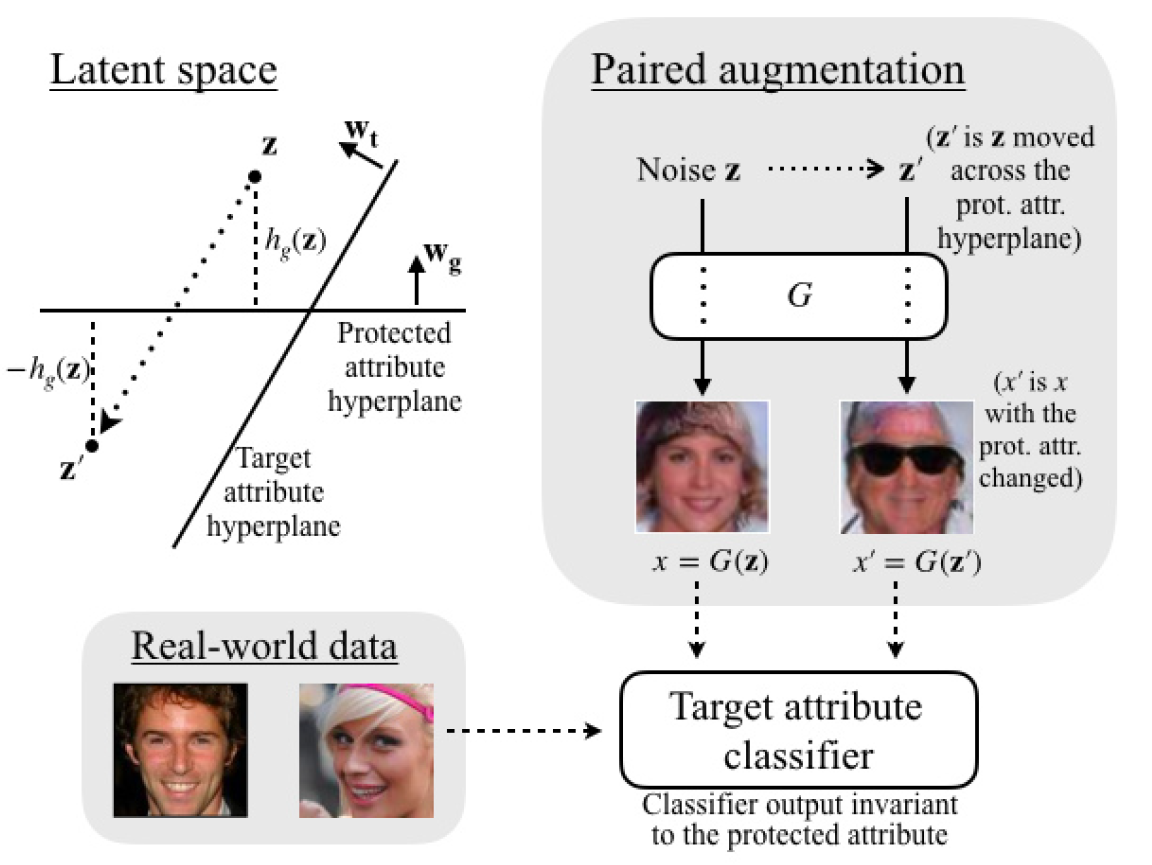
\includegraphics[width=0.5\columnwidth]{./figs/gan.png}
		\end{center}
		\caption{Assume that the latent space is approximately linearly separable. For each latent vector $z$ sampled from the latent space of a trained GAN, we compute $z'$ such that its target attribute score  remains the same (according to $w_t$) while its protected attribute score $h_g(z')$ is negated. Hyperplane is learned by SVM.}
	\end{figure}


\end{frame}

\subsection{In-processing}
\begin{frame}{In-processing Methods}
	\begin{figure}[t]
		\begin{center}
			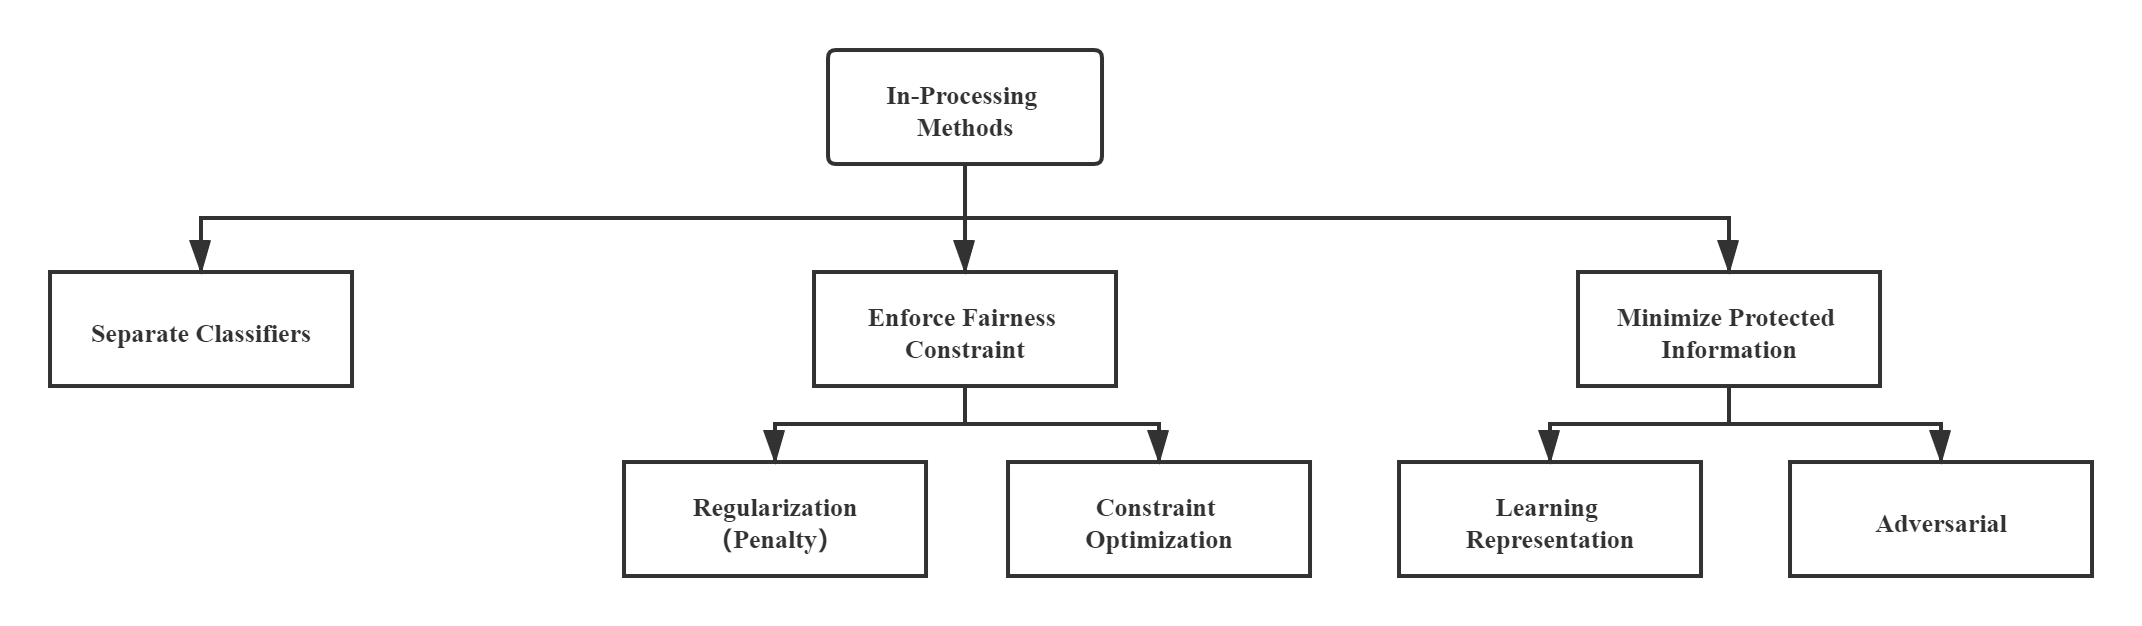
\includegraphics[width=\columnwidth]{./figs/ipm.png}
		\end{center}
		\caption{Classification of In-Processing methods.}
	\end{figure}
\end{frame}
\begin{frame}{Two Naive Bayes}
	\begin{itemize}
		\item Observation: Removing $Z$ from the feature set results in too big of loss in accuracy.
		\item Let $X$ consist of m features  $X=\langle X^{(1)},\cdots,X^{(m)}\rangle$. A model that depends on $Z$ can be formulated as
		      \[P(X,Y|Z)=P(Y|Z)\prod_{i=1}^m P(X^{(i)}|Y,Z)\]

		\item \textbf{Two Naive Bayes:} Train a naive Bayes classifier for each protected attribute and balance them in order to achieve group fairness \cite{calders2010three}.
	\end{itemize}


\end{frame}


\begin{frame}{Prejudice Remover Regularizer}
	\begin{itemize}
		\item To measure prejudice, Kamishima et al. defined the (indirect) prejudice index (PI)
		      \[\text{PI}=\sum_{Y,Z} P(Y,Z)\ln\frac{P(Y,Z)}{P(Y)P(Z)} \]
		\item Let $\Theta$ denote the parameters of the prediction model $h$. The prejudice removing regularization term is defined as \cite{kamishima2012fairness} 
		      \[R_{PR}(D,\Theta)=\sum_{(x,z)\in D}\sum_{y\in \{0,1\}} h(x;\Theta)\ln \frac{P(\hat{Y}=y|Z=z)}{P(\hat{Y}=y)}\]

	\end{itemize}

\end{frame}


\begin{frame}{Learning Fair Representations}
	\begin{itemize}
		\item Map input data into one of $k$ learned prototypes over which the decision takes place.
		\item Let $C$ denote a variable representing one of the prototypes. The probabilistic mapping is defined by
		      \[ P(C=k|X=x)=\frac{\exp(-d(x,v_k))}{\sum_{j=1}^K \exp(-d(x,v_j))}\]
		      where $d(\cdot,\cdot)$ is a distance measure and $v_k$ is a vector associated with each prototype.
		\item The learning system for the prototypes should minimise the loss function \[L=A_CL_C+A_XL_X+A_YL_Y\]
		      where $A_C$, $A_X$ and $A_Y$ are hyperparameters \cite{zafar2017fairness}.

	\end{itemize}

\end{frame}

\begin{frame}{Learning Fair Representations}
	\begin{itemize}
		\item  $L_C$, $L_X$ and $L_Y$ are defined as
		      \begin{align*}
			      L_C & =\sum_{k=1}^K |E(C=k|Z=1)-E(C=k|Z=0)|                            &  & \text{\% Group Fairness} \\
			      L_X & =\sum_{(x,y,z)\in D} \left(x-\sum_{k=1}^k P(C=k|X=x)v_k\right)^2 &  & \text{\% Close to $x$}   \\
			      L_Y & =\sum_{(x,y,z)\in D} -y\log(\hat{y})-(1-y)\log(1-\hat{y})        &  & \text{\% Accuracy}
		      \end{align*}
		      where $\hat{y}=\sum_{k=1}^k P(C=k|X=x)w_k$ and $w_k$ is the probabilistic outcome prediction for prototype $k$.
	\end{itemize}

\end{frame}

\begin{frame}{Learning Fair Representations}
	\begin{figure}[t]
		\begin{center}
			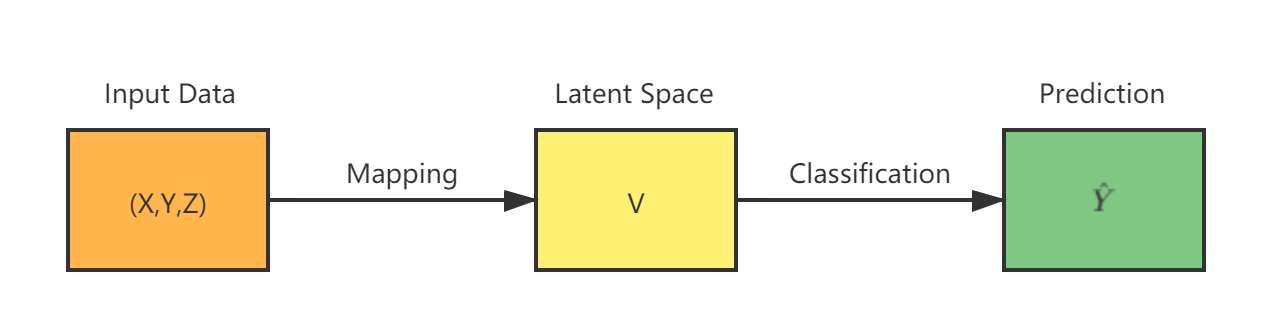
\includegraphics[width=0.8\columnwidth]{./figs/LRF.png}
		\end{center}
		\caption{Workflow of Learning Fair Representation.}
	\end{figure}
	\begin{itemize}
		\item Since $k$ is usually quite large, L-BFGS is employed to minimize the loss function.
	\end{itemize}
\end{frame}

\begin{frame}{Adversarial Learning Fair Representations}
	\begin{figure}[t]
		\begin{center}
			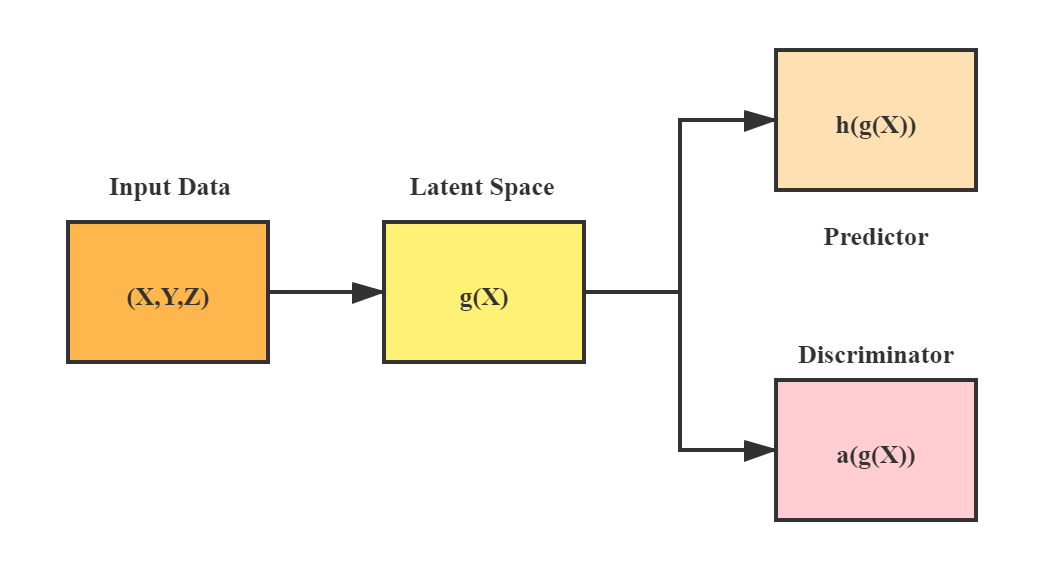
\includegraphics[width=0.6\columnwidth]{./figs/ALRF.png}
		\end{center}
		\caption{Structure of Adversarial  Learning Fair Representation \cite{beutel2017data}.}
	\end{figure}
\end{frame}

\begin{frame}{Adversarial Learning Fair Representations}
	\begin{itemize}
		\item Assume a subset $E=(X_E, Z_E, Y_E)\in D$ from which $Z$ can be observed.
		\item The goal of the predictor model $h(g(X))$ is to correctly predict $Y$ whereas the
		      goal of the discriminator $a(g(XE))$ is to correctly predict $Z$. The overall model’s objective is defined over two loss functions, one for $h$ and $a$ respectively
		      \[\min \sum_{(x,y,z)\in D} L_Y(h(g(x)),y)+\sum_{(x,y,z)\in E} L_Z(a(J_\lambda (g(x))),z)\]
		      where $J_\lambda$ is an identity function with negative gradient, i.e. $J_\lambda(g(X_E))=g(X_E)$ and $\frac{\nabla J_\lambda}{\nabla X_E}=-\lambda \frac{\nabla d(X_E)}{\nabla X_E}$. The $\lambda$ parameter determines the trade-off between accuracy and fairness .
	\end{itemize}
\end{frame}


\begin{frame}{Adversarial Debiasing}
	\begin{figure}[t]
		\begin{center}
			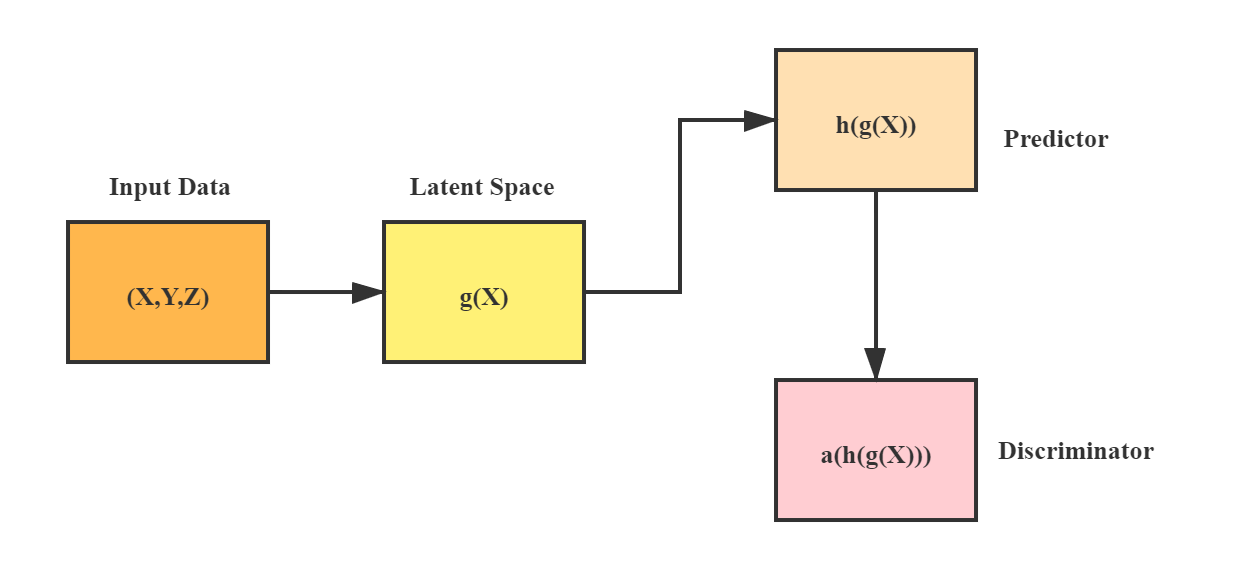
\includegraphics[width=0.8\columnwidth]{./figs/ADB.png}
		\end{center}
		\caption{Structure of Adversarial  Debiasing \cite{zhang2018mitigating}.}
	\end{figure}
\end{frame}

\begin{frame}{Adversarial Debiasing}
	\begin{itemize}
		\item Adversarial Debiasing allows for the notions of group fairness.
		\item Assume the loss functions $L_P(\hat{y},y)$ for the predictor and $L_A(\hat{z},z)$ for the adversary, and the model parameters $W$ and $U$ for predictor and adversary respectively.
		\item $U$ is updated according to the gradient $\nabla_UL_A$.
		\item $W$ is updated according to
		      \[\nabla_WL_P-\text{proj}_{\nabla_W L_A}\nabla_WL_P -\alpha \nabla_WL_A\]
		      where $\alpha $ is a tunable hyperparameter and $\text{proj}_v=0$ if $v=0$.
	\end{itemize}
	Note: If $\nabla_W L_A$ is a unit vector and $\alpha=0$, this update of $W$ leads increase in accuracy but no decrease in fairness.
\end{frame}

\begin{frame}{Constraint Optimization}
	\begin{itemize}
		\item Given a convex decision boundary-based classifier, Zafar et al (2017) propose to minimise loss subject to posed fairness constraints  \cite{zafar2017fairness}.
		\item Zafar et al (2017)  additionally propose a method which, rather than maximising accuracy under fairness constraints, aims to maximise fairness under accuracy constraints \cite{zafar2017fairness2}.
		\item Andrija et al (2021) propose to solve the non-differentiable problem of Group Fairness constraints using Monte Carlo policy gradient method \cite{petrovic2021fair}.

	\end{itemize}
\end{frame}

\subsection{Post-processing}

\begin{frame}{Post-processing}
	\begin{figure}[t]
		\begin{center}
			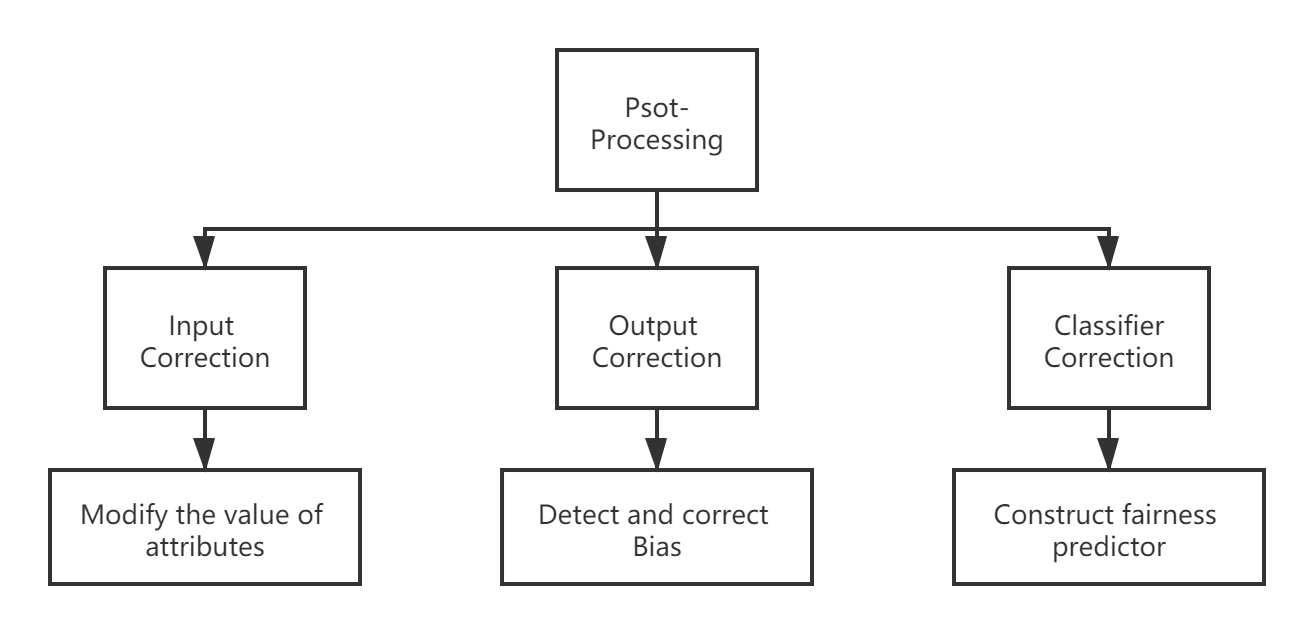
\includegraphics[width=0.8\columnwidth]{./figs/ppm.png}
		\end{center}
		\caption{Overview of Post-processing methods.}
	\end{figure}

\end{frame}



%%%%%%%%%%%%%%%%%%%%%%%%%%%%%%%%%%%%%%%%%%%%%%%%%%%%%%%%%%%%%%%
\section{Recent \& Future Work}

\begin{frame}{Recent works}
	\begin{figure}[t]
		\begin{center}
			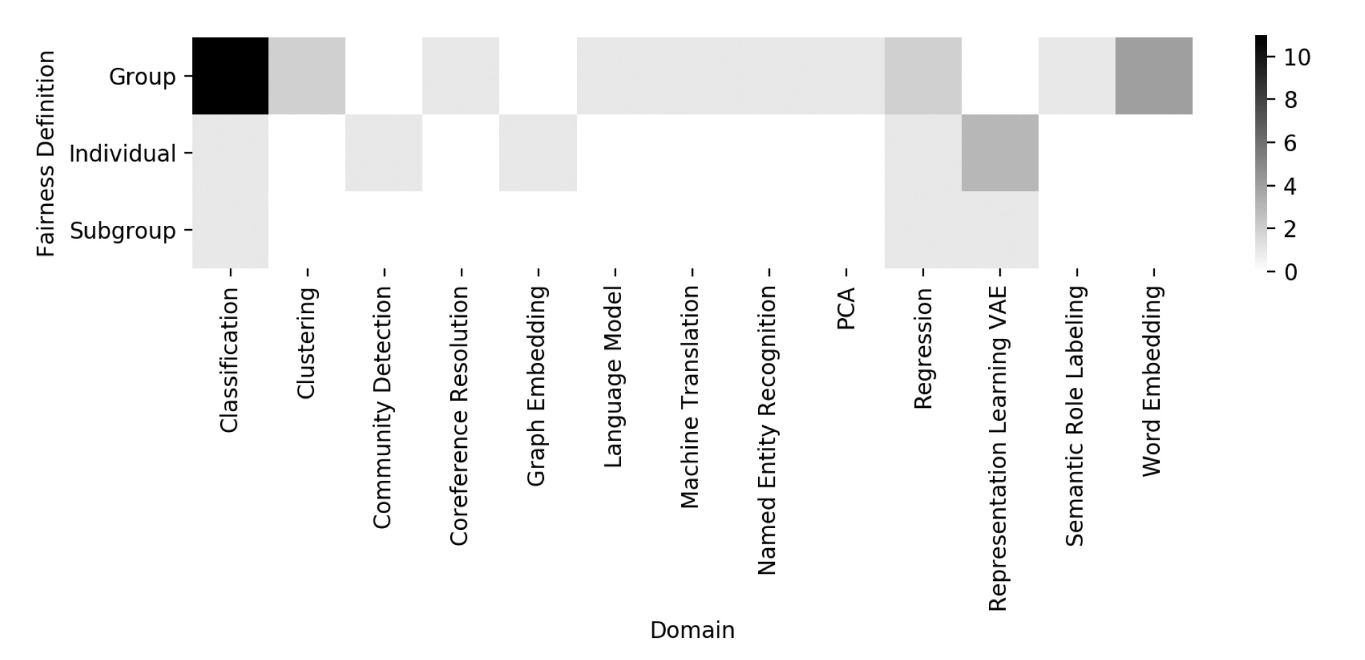
\includegraphics[width=0.8\columnwidth]{./figs/heatmap.png}
		\end{center}
		\caption{Heatmap depicting distribution of previous work in fairness, grouped by domain and fairness definition \cite{mehrabi2021survey}.}
	\end{figure}
\end{frame}

\begin{frame}{Recent works}
	Current works focus on
	\begin{itemize}
		\item Definition of fairness.
		\item Reveal unfairness in Machine Learning.
		\item Achieve fairness in traditional Machine Learning with theoretical guarantee.
		\item Achieve fairness in various deep Learning tasks.
	\end{itemize}
\end{frame}


\begin{frame}{Challenge \& Future works}
	There are several remaining challenges to be addressed in the fairness literature \cite{mehrabi2021survey}. Among them are:
	\begin{itemize}
		\item Synthesizing a definition of fairness: Having a more unified fairness definition and framework can also help with the incompatibility issue of some current fairness definitions.
		\item From Equality to Equity: The definitions presented in the literature mostly focus on equality, ensuring that each individual or group is given the same amount of resources, attention, or outcome. However, little attention has been paid to equity, which is the concept that each	 individual or group is given the resources they need to succeed.
	\end{itemize}
\end{frame}

\begin{frame}{Challenge \& Future works}
	\begin{itemize}
		\item Searching for Unfairness: Given a definition of fairness, it should be possible to identify instances of this unfairness in a particular dataset.
		\item Fairness-aware Optimization in Deep Learning: A few works on adversarial learning have been made. However, fairness-aware optimization process for deep learning receives little attention.
	\end{itemize}
\end{frame}

\section{Q\& A}
\begin{frame}
	\Huge{\centerline{-Q \& A-}}
\end{frame}
\section{Appendix}
\label{app}
\begin{frame}{Tools}
	\begin{table}[]
		\begin{tabular}{|l|l|l|l|}
			\hline
			Name                & Authors                         & Detection & Mitigation \\ \hline
			Fairness Measures   & Zehlike et al., 2017            & Yes       & No         \\ \hline
			FairML              & Adebayo, 2016                   & Yes       & No         \\ \hline
			FairTest            & Tramer et al., 2017             & Yes       & No         \\ \hline
			Aequitas            & Stevens et al., 2018            & Yes       & Yes        \\ \hline
			Themis-ML           & Bantilan, 2018                  & Yes       & Yes        \\ \hline
			Fairness Comparison & Friedler et al., 2018           & Yes       & Yes        \\ \hline
			AF360               & Bellamy, Rachel KE, et al. 2018 & Yes       & Yes        \\ \hline
		\end{tabular}
		\caption{Tools for Fairness in ML.}
	\end{table}
\end{frame}


\begin{frame}{Criteria of Fairness}
	Many fairness criterias have been proposed over the years that can generally be divided into three categories:
	\begin{itemize}
		\item Individual Fairness: Give similar predictions to similar individuals.
		\item Group Fairness: Treat different groups equally.
		\item Subgroup Fairness: Subgroup fairness intends to obtain the best properties of the group	and individual notions of fairness. It is different than these notions but uses them to obtain better outcomes. It picks a group fairness constraint like equalizing false positive and asks whether this constraint holds over a large collection of subgroups.
	\end{itemize}

\end{frame}
\begin{frame}{Criteria of Fairness}
	Most of the proposed fairness criterias are properties of the joint distribution of the sensitive attribute A, the target label Y, and the	predicated label $\hat{Y}$. Here we assume that $Y, A\in \{0,1\}$ and give the definition of some popular measures summarized in \cite{mehrabi2021survey}.
	\begin{definition}[Equalized Odds]
		An algorithm is fair if
		$$ P(\hat{Y}|A=0,Y=y)=P(\hat{Y}|A=1,Y=y)$$
	\end{definition}
	\begin{definition}[Equal Opportunity]
		An algorithm is fair if
		$$ P(\hat{Y}=1|A=0,Y=1)=P(\hat{Y}=1|A=1,Y=1)$$
	\end{definition}

\end{frame}

\begin{frame}{Criteria of Fairness}
	\begin{definition}[Demographic Parity]
		An algorithm is fair if
		$$ P(\hat{Y}|A=0)=P(\hat{Y}|A=1)$$
	\end{definition}
	\begin{definition}[Fairness through Awareness]
		An algorithm is fair if it gives similar predictions to
		similar individuals.
	\end{definition}

	\begin{definition}[Fairness through Unawareness]
		An algorithm is fair as long as any protected attributes
		A are not explicitly used in the decision-making process.
	\end{definition}

\end{frame}

\begin{frame}{Criteria of Fairness}
	\begin{definition}[Treatment Equality]
		The ratio of false negatives and false positives is the same for both protected group categories.
	\end{definition}
	\begin{definition}[Test Fairness]
		For any predicted probability score S, people in both protected and unprotected groups must have equal probability of correctly belonging to the positive class.
	\end{definition}

	\begin{definition}[Counterfactual Fairness]
		A decision is fair towards an individual if it is the same in both the actual world and a counterfactual world where the individual belonged to a different demographic group.
	\end{definition}

\end{frame}

\begin{frame}{Criteria of Fairness}
	\begin{definition}[Fairness in Relational Domains]
		A notion of fairness that is able to capture the
		relational structure in a domain—not only by taking attributes of individuals into consideration
		but by taking into account the social, organizational, and other connections between individuals.
	\end{definition}
	\begin{definition}[Conditional Statistical Parity]
		People in both protected and unprotected (female and male) groups should have equal probability of being assigned to a positive outcome given a set of legitimate factors L.
	\end{definition}

\end{frame}
\begin{frame}{Current works}
	\begin{figure}[t]
		\begin{center}
			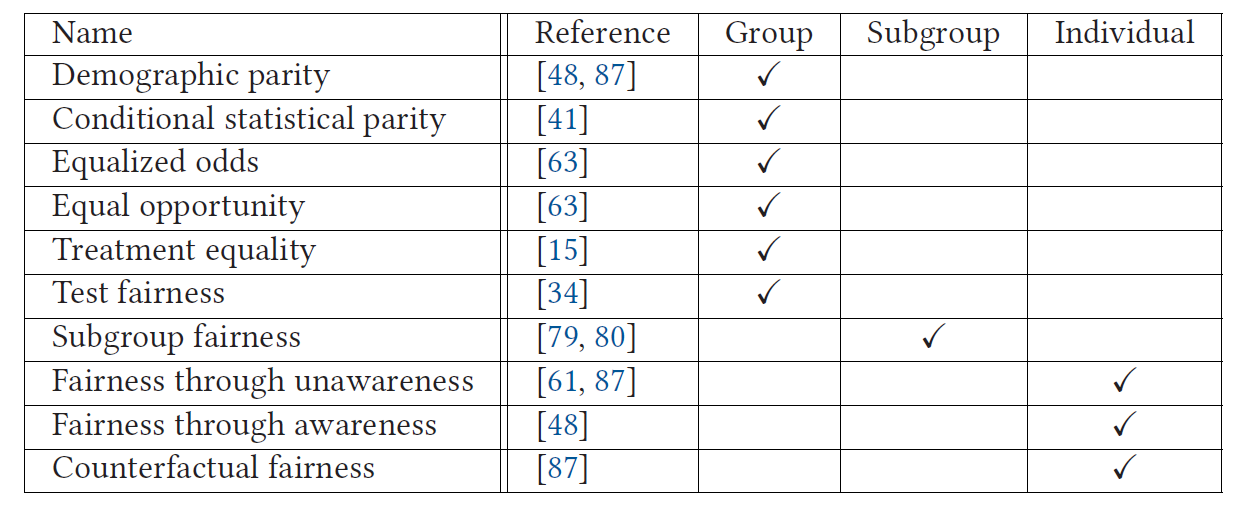
\includegraphics[width=0.8\columnwidth]{./figs/fairness_def.png}
		\end{center}
		\caption{Categorizing Different Fairness Notions into Group, Subgroup, and Individual Types \cite{mehrabi2021survey}.}
	\end{figure}
\end{frame}


\begin{frame}{Current Works}
	\begin{figure}[t]
		\begin{center}
			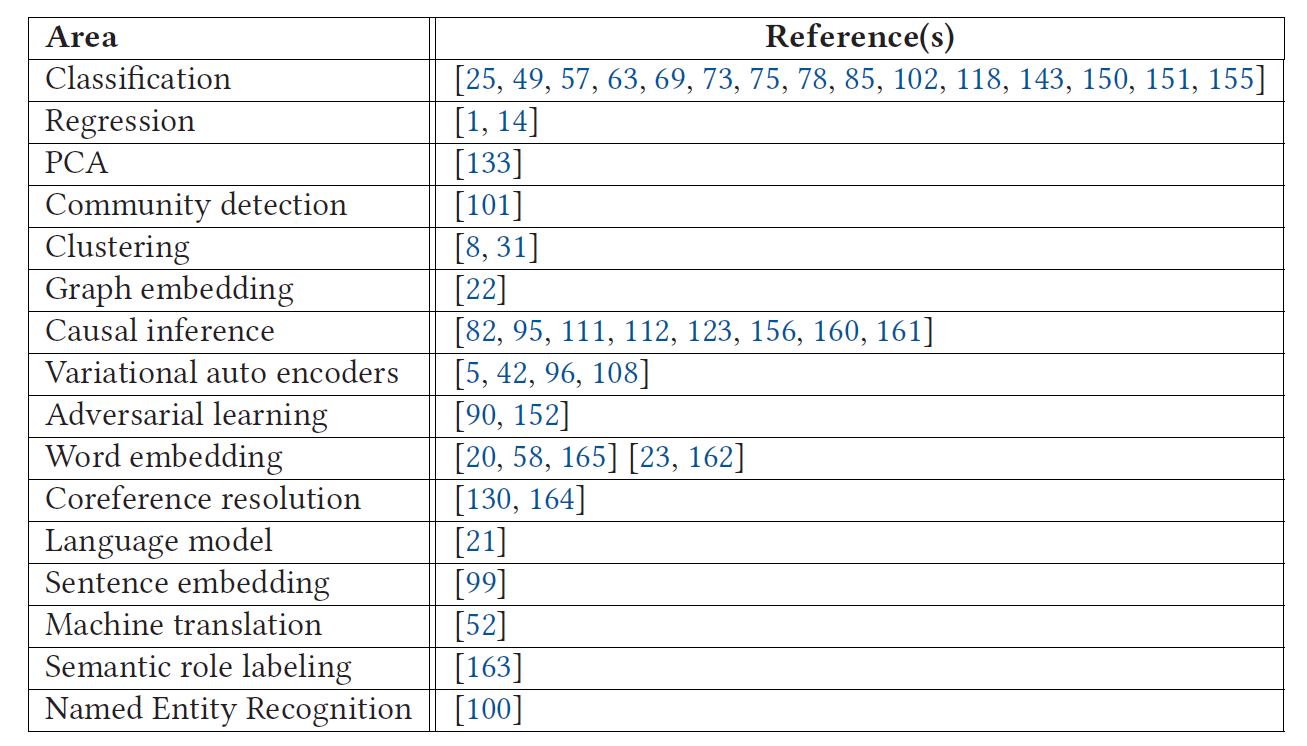
\includegraphics[width=0.6\columnwidth]{./figs/list_mlf.png}
		\end{center}
		\caption{List of Papers Targeting and Talking about Bias and Fairness in Different Areas \cite{mehrabi2021survey}.}
	\end{figure}
\end{frame}

\begin{frame}{Dataset}
	\begin{figure}[t]
		\begin{center}
			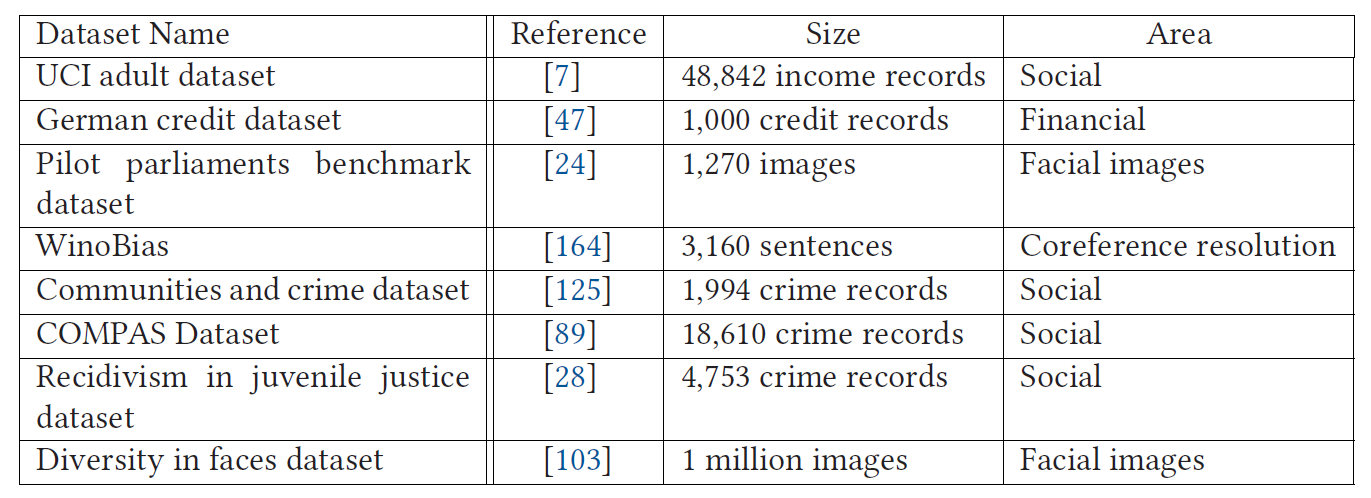
\includegraphics[width=0.8\columnwidth]{./figs/dataset.png}
		\end{center}
		\caption{Most Widely Used Datasets in the Fairness Domain with Additional Information about Each of the Datasets Including Their Size and Area of Concentration \cite{mehrabi2021survey}.}
	\end{figure}
\end{frame}

\begin{frame}{Dataset}
	\begin{itemize}
		\item FairFace \cite{karkkainen2021fairface}:  A novel face image dataset containing 108,501 images which is balanced on race.
	\end{itemize}

\end{frame}

\begin{frame}{Procedure for Fairness Research}
	\begin{itemize}
		\item Identify the protected attribute and target label.
		\item Identify the type of bias/discrimination in dataset, e.g. underrepresentation of certain group or indirect discrimination to protect attributes.
		\item Identify the definition of fairness and criteria.
		\item Identify the phase new methods target.
	\end{itemize}

\end{frame}

%\begin{frame}
%	\frametitle{References}
%	\footnotesize{
%		\begin{thebibliography}{99} % Beamer does not support BibTeX so references must be inserted manually as below
%			\bibitem[Zhang, H. and Davidson, I., 2021]{zhang2021towards} Zhang, Hongjing and Davidson, Ian (2021)
%			\newblock Towards Fair Deep Anomaly Detection
%			\newblock \emph{Proceedings of the 2021 ACM Conference on Fairness, Accountability, and Transparency} 138--148.
%
%			\bibitem[mehrabi2021survey, 2021]{mehrabi2021survey} Mehrabi, Ninareh and Morstatter, Fred and Saxena, Nripsuta and Lerman, Kristina and Galstyan, Aram (2021)
%			\newblock A survey on bias and fairness in machine learning
%			\newblock \emph{ACM Computing Surveys (CSUR)} 54(6), 1--35.
%
%			\bibitem[barocas2017fairness, 2017]{barocas2017fairness} Barocas, Solon and Hardt, Moritz and Narayanan, Arvind (2017)
%			\newblock Fairness in machine learning
%			\newblock \emph{Nips tutorial} 1
%
%			\bibitem[bellamy2018ai, 2018]{bellamy2018ai} Bellamy, Rachel KE and Dey, Kuntal and Hind, Michael and Hoffman, Samuel C and Houde, Stephanie and Kannan, Kalapriya and Lohia, Pranay and Martino, Jacquelyn and Mehta, Sameep and Mojsilovic, Aleksandra and others (2018)
%			\newblock AI Fairness 360: An extensible toolkit for detecting, understanding, and mitigating unwanted algorithmic bias
%			\newblock \emph{arXiv preprint arXiv:1810.01943}
%
%		\end{thebibliography}
%	}
%\end{frame}


\begin{frame}[t, allowframebreaks]
\frametitle{References}
\footnotesize
\bibliographystyle{amsalpha}
\bibliography{reference.bib}
\end{frame}

\end{document}
